%%%%%%%%%%%%%%%%%%%%%%%%%%%%%%%%%%%%%%%%%%%%%%%%%%%%%%%%%%%%%%%%%%%%
%% I, the copyright holder of this work, release this work into the
%% public domain. This applies worldwide. In some countries this may
%% not be legally possible; if so: I grant anyone the right to use
%% this work for any purpose, without any conditions, unless such
%% conditions are required by law.
%%%%%%%%%%%%%%%%%%%%%%%%%%%%%%%%%%%%%%%%%%%%%%%%%%%%%%%%%%%%%%%%%%%%

\documentclass[
  digital,     %% The `digital` option enables the default options for the
               %% digital version of a documeant. Replace with `printed`
               %% to enable the default options for the printed version
               %% of a document.
%%  color,       %% Uncomment these lines (by removing the %% at the
%%               %% beginning) to use color in the printed version of your
%%               %% document
  oneside,     %% The `oneside` option enables one-sided typesetting,
               %% which is preferred if you are only going to submit a
               %% digital version of your thesis. Replace with `twoside`
               %% for double-sided typesetting if you are planning to
               %% also print your thesis. For double-sided typesetting,
               %% use at least 120 g/m² paper to prevent show-through.
  nosansbold,  %% The `nosansbold` option prevents the use of the
               %% sans-serif type face for bold text. Replace with
               %% `sansbold` to use sans-serif type face for bold text.
  nocolorbold, %% The `nocolorbold` option disables the usage of the
               %% blue color for bold text, instead using black. Replace
               %% with `colorbold` to use blue for bold text.
  nolof,         %% The `lof` option prints the List of Figures. Replace
               %% with `nolof` to hide the List of Figures.
  nolot,         %% The `lot` option prints the List of Tables. Replace
               %% with `nolot` to hide the List of Tables.
]{fithesis4}
%% The following section sets up the locales used in the thesis.
\usepackage[resetfonts]{cmap} %% We need to load the T2A font encoding
\usepackage[T1,T2A]{fontenc}  %% to use the Cyrillic fonts with Russian texts.
\usepackage[
  main=english, %% By using `czech` or `slovak` as the main locale
                %% instead of `english`, you can typeset the thesis
                %% in either Czech or Slovak, respectively.
  english, german, russian, czech, slovak %% The additional keys allow
]{babel}        %% foreign texts to be typeset as follows:
%%
%%   \begin{otherlanguage}{german}  ... \end{otherlanguage}
%%   \begin{otherlanguage}{russian} ... \end{otherlanguage}
%%   \begin{otherlanguage}{czech}   ... \end{otherlanguage}
%%   \begin{otherlanguage}{slovak}  ... \end{otherlanguage}
%%
%% For non-Latin scripts, it may be necessary to load additional
%% fonts:
\usepackage{paratype}
\usepackage{todonotes}
\setuptodonotes{inline}
\def\textrussian#1{{\usefont{T2A}{PTSerif-TLF}{m}{rm}#1}}
%%
%% The following section sets up the metadata of the thesis.
\thesissetup{
    date        = \the\year/\the\month/\the\day,
    university  = mu,
    faculty     = fi,
    type        = bc,
    department  = Department of Computer Systems and Communications,
    author      = Tomáš Marek,
    gender      = f,
    advisor     = {Ing. Milan Brož, Ph.D.},
    title       = {Improvements of the Randomness Testing Toolkit},
    TeXtitle    = {Improvements of the Randomness Testing Toolkit},
    keywords    = {keyword1, keyword2, ...},
    TeXkeywords = {keyword1, keyword2, \ldots},
    abstract    = {%
      This is the abstract of my thesis, which can

      span multiple paragraphs.
    },
    thanks      = {%
      These are the acknowledgements for my thesis, which can

      span multiple paragraphs.
    },
    bib         = bibliography.bib,
    %% Remove the following line to use the JVS 2018 faculty logo.
    facultyLogo = fithesis-fi,
}
\usepackage{makeidx}      %% The `makeidx` package contains
\makeindex                %% helper commands for index typesetting.
%% These additional packages are used within the document:
\usepackage{paralist} %% Compact list environments
\usepackage{amsmath}  %% Mathematics
\usepackage{amsthm}
\usepackage{amsfonts}
\usepackage{url}      %% Hyperlinks
\usepackage{markdown} %% Lightweight markup
\usepackage{listings} %% Source code highlighting
\lstset{
  basicstyle      = \ttfamily,
  identifierstyle = \color{black},
  keywordstyle    = \color{blue},
  keywordstyle    = {[2]\color{cyan}},
  keywordstyle    = {[3]\color{olive}},
  stringstyle     = \color{teal},
  commentstyle    = \itshape\color{magenta},
  breaklines      = true,
}
\usepackage{floatrow} %% Putting captions above tables
\floatsetup[table]{capposition=top}
\usepackage[babel]{csquotes} %% Context-sensitive quotation marks
\begin{document}
%% The \chapter* command can be used to produce unnumbered chapters:
\chapter*{Introduction}
%% Unlike \chapter, \chapter* does not update the headings and does not
%% enter the chapter to the table of contents. I we want correct
%% headings and a table of contents entry, we must add them manually:
\markright{\textsc{Introduction}}
\addcontentsline{toc}{chapter}{Introduction}
\todo{To be done, now it is only a collection of ideas.}

%Random number generators are tested by taking an output sample. This 

The desired properties of random sequence are \emph{uniformity} (for each bit the probability for both zero and one are exactly $1/2$), \emph{independence} (none of the bits is influenced by any other bit) and \emph{unpredictability} (it is impossible to predict next bit by obtaining any number of previous bits). \cite[p. 1-1]{nist_special}

% RANDOMNESS TESTING - 'theoretical' chapter

\chapter{Randomness testing}

Goal of this chapter is to provide overview of randomness testing process and to explain all used terms. Explanations of both one and two level tests are accompanied by example applications.

\section{Overview / Introduction} \label{chap:rand-intro}

%Testing a sequence (define) (tu01guide - 1, tu01paper - 3, 17), required properties(nistspecial 1-1, 1-3 )

During a randomness test a \emph{random sequence} is tested. In this document, a random sequence is a finite sequence of zero and one bits, which was generated by a tested random number generator.  \cite[p. 1-1]{nist_special} 

%Null/alternative hypothesis (tu01paper - 3, možná učebnice)
%Randomness testing as statistical testing (tu01guide - 2)

Randomness test is a form of \emph{empirical statistical test}, where we test our assumption about the tested data - the \emph{null hypothesis} ($H_0$). During the randomness test it states that the sequence is \emph{random}. Associated with the null-hypothesis is the \emph{alternative hypothesis} ($H_1$), which states that the sequence is \emph{non-random}. Goal of the test is to search for evidence against the null-hypothesis. \cite[p. 2]{tu01_guide}

%Idea of testing – extremeness of a sample ? (nistspecial - 1-3+)

%result (accept, reject, Type I/II error) (nistspecial - 1-3+, učebnice 416)

The result of the test is either that we \emph{accept} the null hypothesis (the sequence is considered random), or that we \emph{reject} the null-hypothesis (and accept the alternative hypothesis - the sequence is considered non-random). We reject the null hypothesis when the evidence found against the null-hypothesis is strong enough, otherwise we accept it. Based on the true situation of null hypothesis, four situations depicted in Table \ref{tab:type_errors} may occur. \cite[p. 417]{basic_practice}

\begin{table}
  \begin{tabularx}{0.7\textwidth}{l|c|c}
    %\toprule
    TRUE  & \multicolumn{2}{c}{TEST CONCLUSION}\\
    SITUATION &Accept $H_0$ & Reject $H_0$\\
    \midrule
    $H_0$ is True &  No error & Type I error  \\
    $H_0$ is False & Type II error & No error \\
    %\bottomrule
  \end{tabularx}
  \caption{Possible outcomes when assessing the result of statistical test.}
  \label{tab:type_errors}
\end{table}

\section{Single-level testing} \label{chap:rand-single}
%significance level (tu01 paper 5-8, nistspecial 1-3+, rec for stat testing 5, učebnice)

A single-level test examines the random sequence directly (compare with \ref{chap:rand-two_level}). Before the test user must choose a \emph{significance level}, which determines how strong the found evidence has to be to reject the null-hypothesis. The test yields a \emph{p-value}, which is used to make the accept or reject the null-hypothesis.

The \emph{significance level} ($\alpha$) is crucial to assessing the test result and must be set before the test. The $\alpha$ is equal to probability of Type I Error. Usual values are $\alpha = 0.05$ or $\alpha = 0.01$ \cite[p. 390]{basic_practice}, for use in testing of cryptographic random number generators lower values may be chosen. \cite[p. 1-4]{nist_special} The lower $\alpha$ is set, the stronger the found evidence has to be to reject the null hypothesis. %(cite? derived from nistspecial 1-4)

%Test statistic (= function, known distribution), sample (tu01 paper 4+)

The randomness test is defined by a \emph{test statistic} $Y$, which is a function of a finite bit sequence. Distribution of its values under the null hypothesis must be known (or at least approximated). The value of the test statistic ($y$) is computed for the tested random sequence. Each test statistic searches for presence or absence of some "pattern" in the sequence, which would show the non-randomness of the sequence. There is infinite number of possible test statistics. \cite[p. 4]{tu01_paper}

%p-value (one, two tailed, how extremeness is set) (nist-opt 5, nist-special 1-4,rec for stat testing 5)

The \emph{p-value} is the probability of the test statistic $Y$ taking value at least as extreme as the observed $y$, assuming that the null hypothesis is true. In randomness testing it is equal to the probability that \emph{perfect random number generator} would generate less random sequence. The smaller is the p-value, the stronger is the found evidence against the null-hypothesis. \cite[p. 386]{basic_practice} The p-value is calculated based on the observed $y$.



\subsection{Result interpretation} \label{chap:rand-interpretation}
%interpratation (učebnice 380-400)

Decision about the test result is based on the computed \emph{p-value}. If the p-value is lower than the $\alpha$, we \emph{reject the null hypothesis} (and accept the alternative hypothesis), because strong enough evidence against null hypothesis was found. If the p-value is greater than or equal to the $\alpha$, we \emph{accept the null hypothesis}, because the evidence against the randomness was too weak. \cite[p. 390]{basic_practice} It is sometimes recommended to report the \emph{p-value} as well instead of accept/reject only, as it yields more information. \cite[p. 90]{tu01_guide}

% TODO: note on moving alpha, for one alpha fail, for other pass

The p-values close to $\alpha$ can be considered \emph{suspicious}, because they do not clearly indicate rejection. Further testing of the random number generator on \emph{other} random sequences is then in place to search for further evidence. \cite[p. 5]{tu01_paper} The reason is that \emph{randomness} is a probabilistic property, therefore even the perfect random number generator may generate a nonrandom sequence with low p-value (although it is very unlikely). The further evidence is used to differentiate between the bad generator generating a non-random sequence systematicaly and the good generator generating non-random sequence 'by chance'. \cite[p. 90]{tu01_guide}

%example
\subsection{Example} \label{chap:rand-example}

To demonstrate how a single randomness test is made, the Frequency (Monobit) Test from NIST STS battery was chosen. \cite[p. 2-2]{nist_special} This test is based on testing the fraction of zeroes and ones within the sequence. For a random sequence with length $n$ the  count of ones (and zeroes) is expected to be around $n/2$ (the most probable values are close to $n/2$). 

For the Monobit test it is recommended that the tested sequence has at least 100 bits. The test statistic $S_{obs}$ of the Monobit test is defined as \[S_{obs} = \dfrac{|\#_1 - \#_0|}{\sqrt{n}}\] where $\#_1$ is count of ones in the tested sequence (similarly for zeroes) and $n$ is length of of the tested sequence. Under the null hypothesis, the reference distribution of $S_{obs}$ is half normal (for large $n$). The p-vaue is computed as \[ p = erfc(\dfrac{S_{obs}}{\sqrt{2}}) \] where $erfc$ is the \emph{complementary error function} used to calculate probabilities in normal distribution.

 Let
\[\begin{split}
    \epsilon = 10011001010010000010001001011001101100001101000111\\10101001010010010011100111001100110010010100111011
\end{split}\]
 be the tested sequence. The test statistic for this sequence is 
 \[S_{obs} = \dfrac{|46 - 54|}{\sqrt{100}}\ = \dfrac{|-8|}{10} = 0.8\]
 and the p-value (visualised at Figure \ref{fig:example}) is 
 \[p = erfc\biggl(\dfrac{0.8}{\sqrt{2}}\biggr) \approx 0.423\]

To interpret the test, we compare the computed \emph{p-value} to the chosen $\alpha$. The $\emph{p-value} \approx 0.423$ is greater than both usual $\alpha = 0.05$ and $\alpha = 0.01$, therefore we accept the null hypothesis for both \emph{significance levels} and the sequence $\epsilon$ is considered random.

\begin{figure}
  \begin{center}
    %% minimus is about 100 pixels per 1 centimeter or 300 pixels per 1 inch.
    %% The optimum is about 250 pixels per 1 centimeter 
    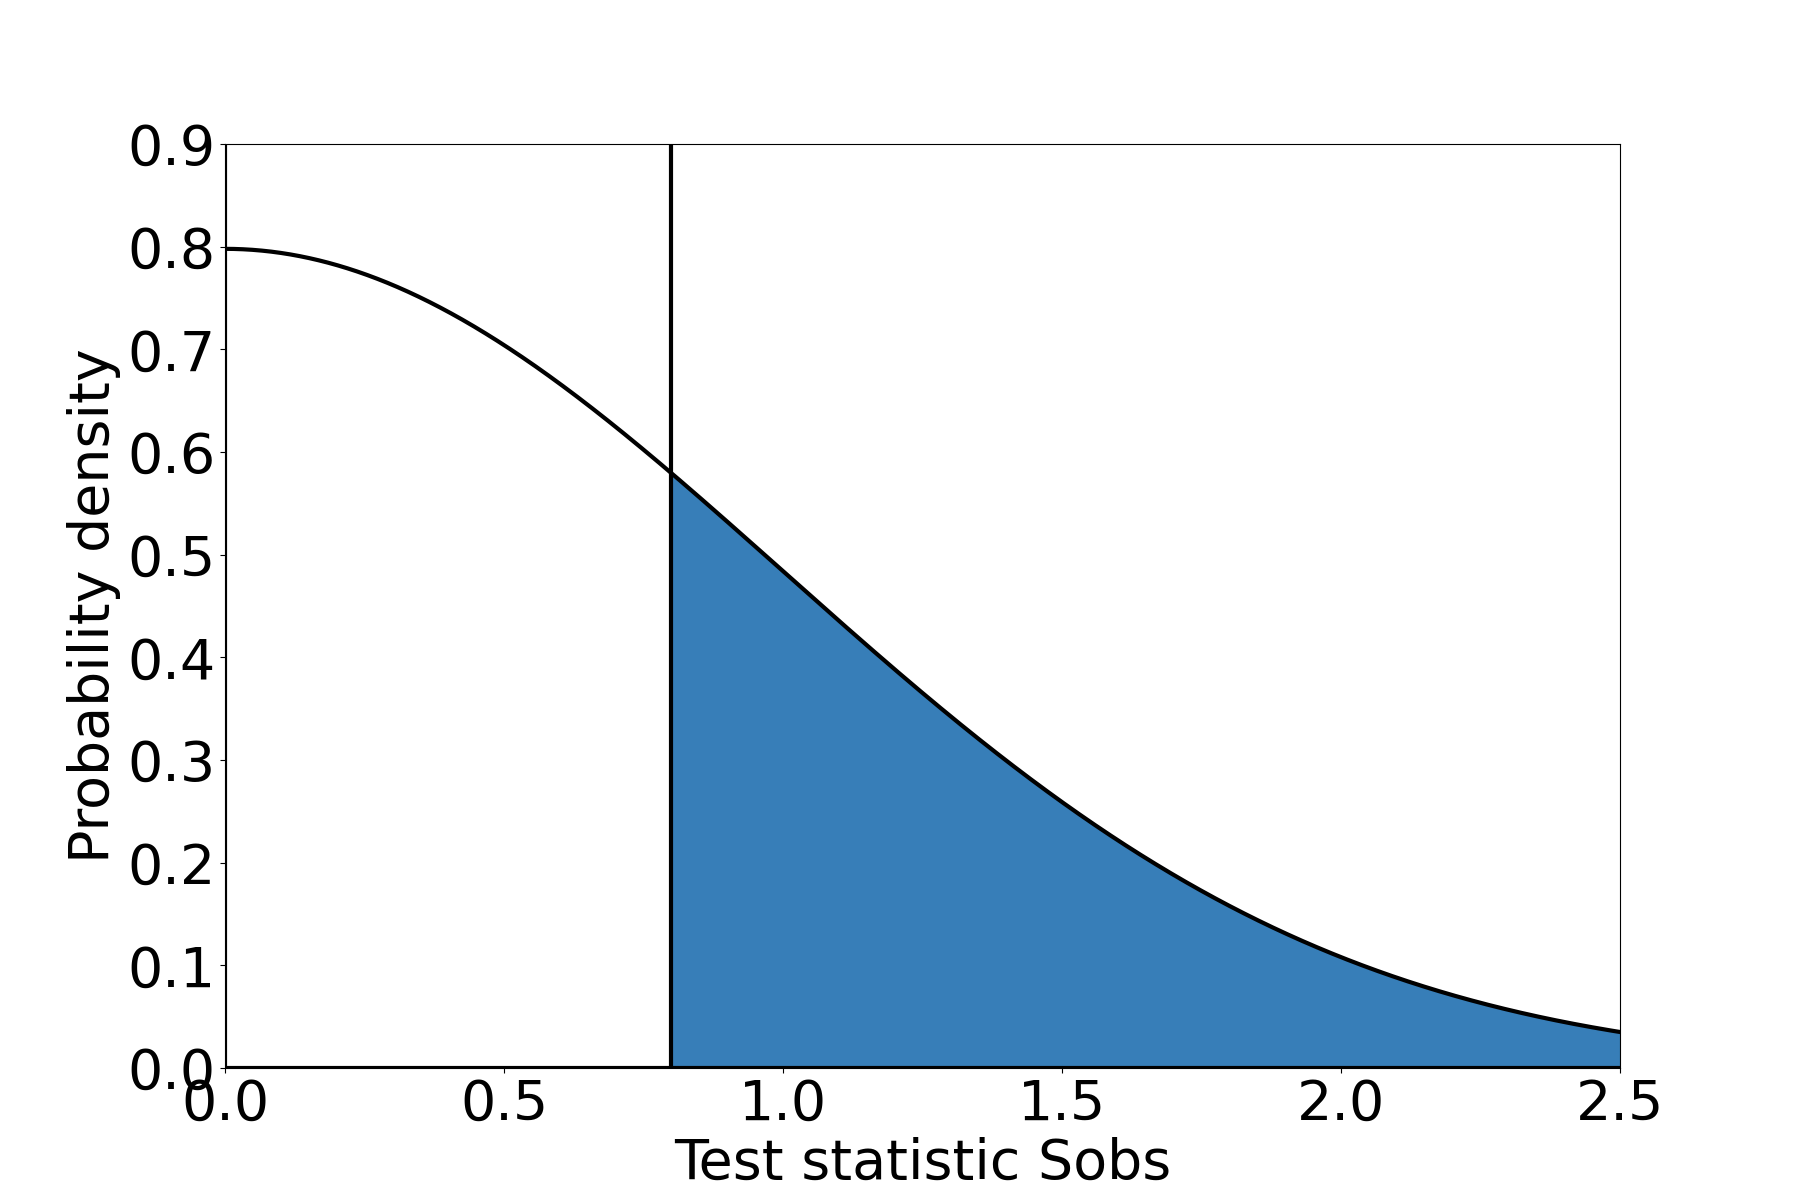
\includegraphics[width=8cm]{figures/test_example.png}
  \end{center}
  \caption{Visualization of example p-value for test statistic value $y = 0.8$}
  \label{fig:example}
\end{figure}

% two-level (tu01guide 88, tu01paper 5-8, correcting_dieharder 14)
\section{Two-level testing} \label{chap:rand-two_level}

% two-level motivation (tu01_paper 5-8)
The \emph{two-level test} is done by repeating the single-level test $n$ times. The important part is comparing the distribution of produced p-values to the expected distribution. The two-level test allows the random sequence to be examined both locally and globally, while the single-level test examines the sequence only on the global level. This may lead to discovering local patterns, which cancel out on the global level. \cite[p. 7]{tu01_paper}

To apply the two-level test the tested sequence is split into $n$ equal-length disjoint subsequences. The same single-level test is applied to each of the subsequences (as described in Section \ref{chap:rand-single}) and its \emph{p-values} are collected, resulting in set of $n$ \emph{p-values}\footnote{Note that the p-values are not subject to accept/reject decision.}. The tests are called \emph{first-level tests} and the p-values are called \emph{first-level p-values}. Under the null-hypothesis, the first-level p-values of a given test statistic are uniformly distributed over the interval $(0,1]$. \cite[p. 14]{bad_day} 

% GOF  - 1
The crucial part of two-level test is examining the distribution of \emph{observed first-level p-values}. Usually, the \emph{goodness-of-fit} (GOF) tests are applied as the \emph{second-level test}. \cite[p. 6]{tu01_paper} GOF tests are a family of methods used for examining how well a data sample fits given distribution. \cite[p. 1]{GOF-techniques} The most used GOF tests in randomness testing are the $\chi^2$ (chi-squared) and Kolmogorov-Smirnov test, another notable tests are the Anderson-Darling and Cramér-von-Mises test. \cite[p. 14]{bad_day}

The second-level test is defined by a test statistic $Y$, which is a function of the first-level p-values. Test statistic value ($y$) is calculated from the observed \emph{first-level p-values} and then the \emph{second-level p-value} is calculated from $y$. At last, the second-level p-value is interpreted as in one-level test (as described in Subsection \ref{chap:rand-interpretation}). 

% ratio of passed sequences
Alternatively, a \emph{proportion of subsequences passing the first-level test} is used to examine the fist-level p-values uniformity. Under the null-hypothesis, it is expected for $n\cdot\alpha$ subsequences to \emph{be rejected} (i.e. to have p-value $< \alpha$) by the first-level test (be a subject to Type I Error). The ratio of sequences passing the first-level test is expected to be around $1-\alpha$, different ratio indicates non-uniformity of observed first-level p-values. \cite[p. 4-2]{nist_special} No p-value is reported in this case, only the ratio.

% GOF comparison?: (rec_for_stat 6)

% KS - description - (para and non para - 171)
\subsection{Kolmogorov-Smirnov test}
The one-sample Kolmogorov-Smirnov (KS) test is used in randomness testing to compare the observed first-level p-values to the uniform distribution. The Kolmogorov-Smirnov test is built on comparing the cumulative distribution function (CDF)\footnote{For a given distribution and value $x$, the CDF returns the probability of drawing a value less than or equal to $x$.} of the expected distribution and the empirical cumulative distribution function (eCDF)\footnote{For a set of observed data and value $x$, the eCDF returns the probability of drawing a value less than or equal to $x$.} of the observed samples. %cdf - nist_special 1-5 

In first variant, two test statistics are calculated. The test statistic $D^+$ ($D^-$) is the maximal vertical distance between CDF and eCDF above (under) the CDF. In second variant, only the test statistic $D$ (maximal vertical distance between CDF and eCDF) is measured. Formally, the test statistics are defined as
\[\begin{split}
    &D^+ = sup_x\{F_n(x) - F(x)\}\\
    &D^- = sup_x\{F(x) - F_n(x)\}\\
    &D \:\:\:= sup_x\{|F_n(x) - F(x)|\} = max(D^+, D^-)
\end{split}
\] where $F(x)$ is the CDF and $F_n(x)$ is the  eCDF \cite[p. 100]{GOF-techniques}.


\begin{figure}
  \begin{center}
    %% minimus is about 100 pixels per 1 centimeter or 300 pixels per 1 inch.
    %% The optimum is about 250 pixels per 1 centimeter 
    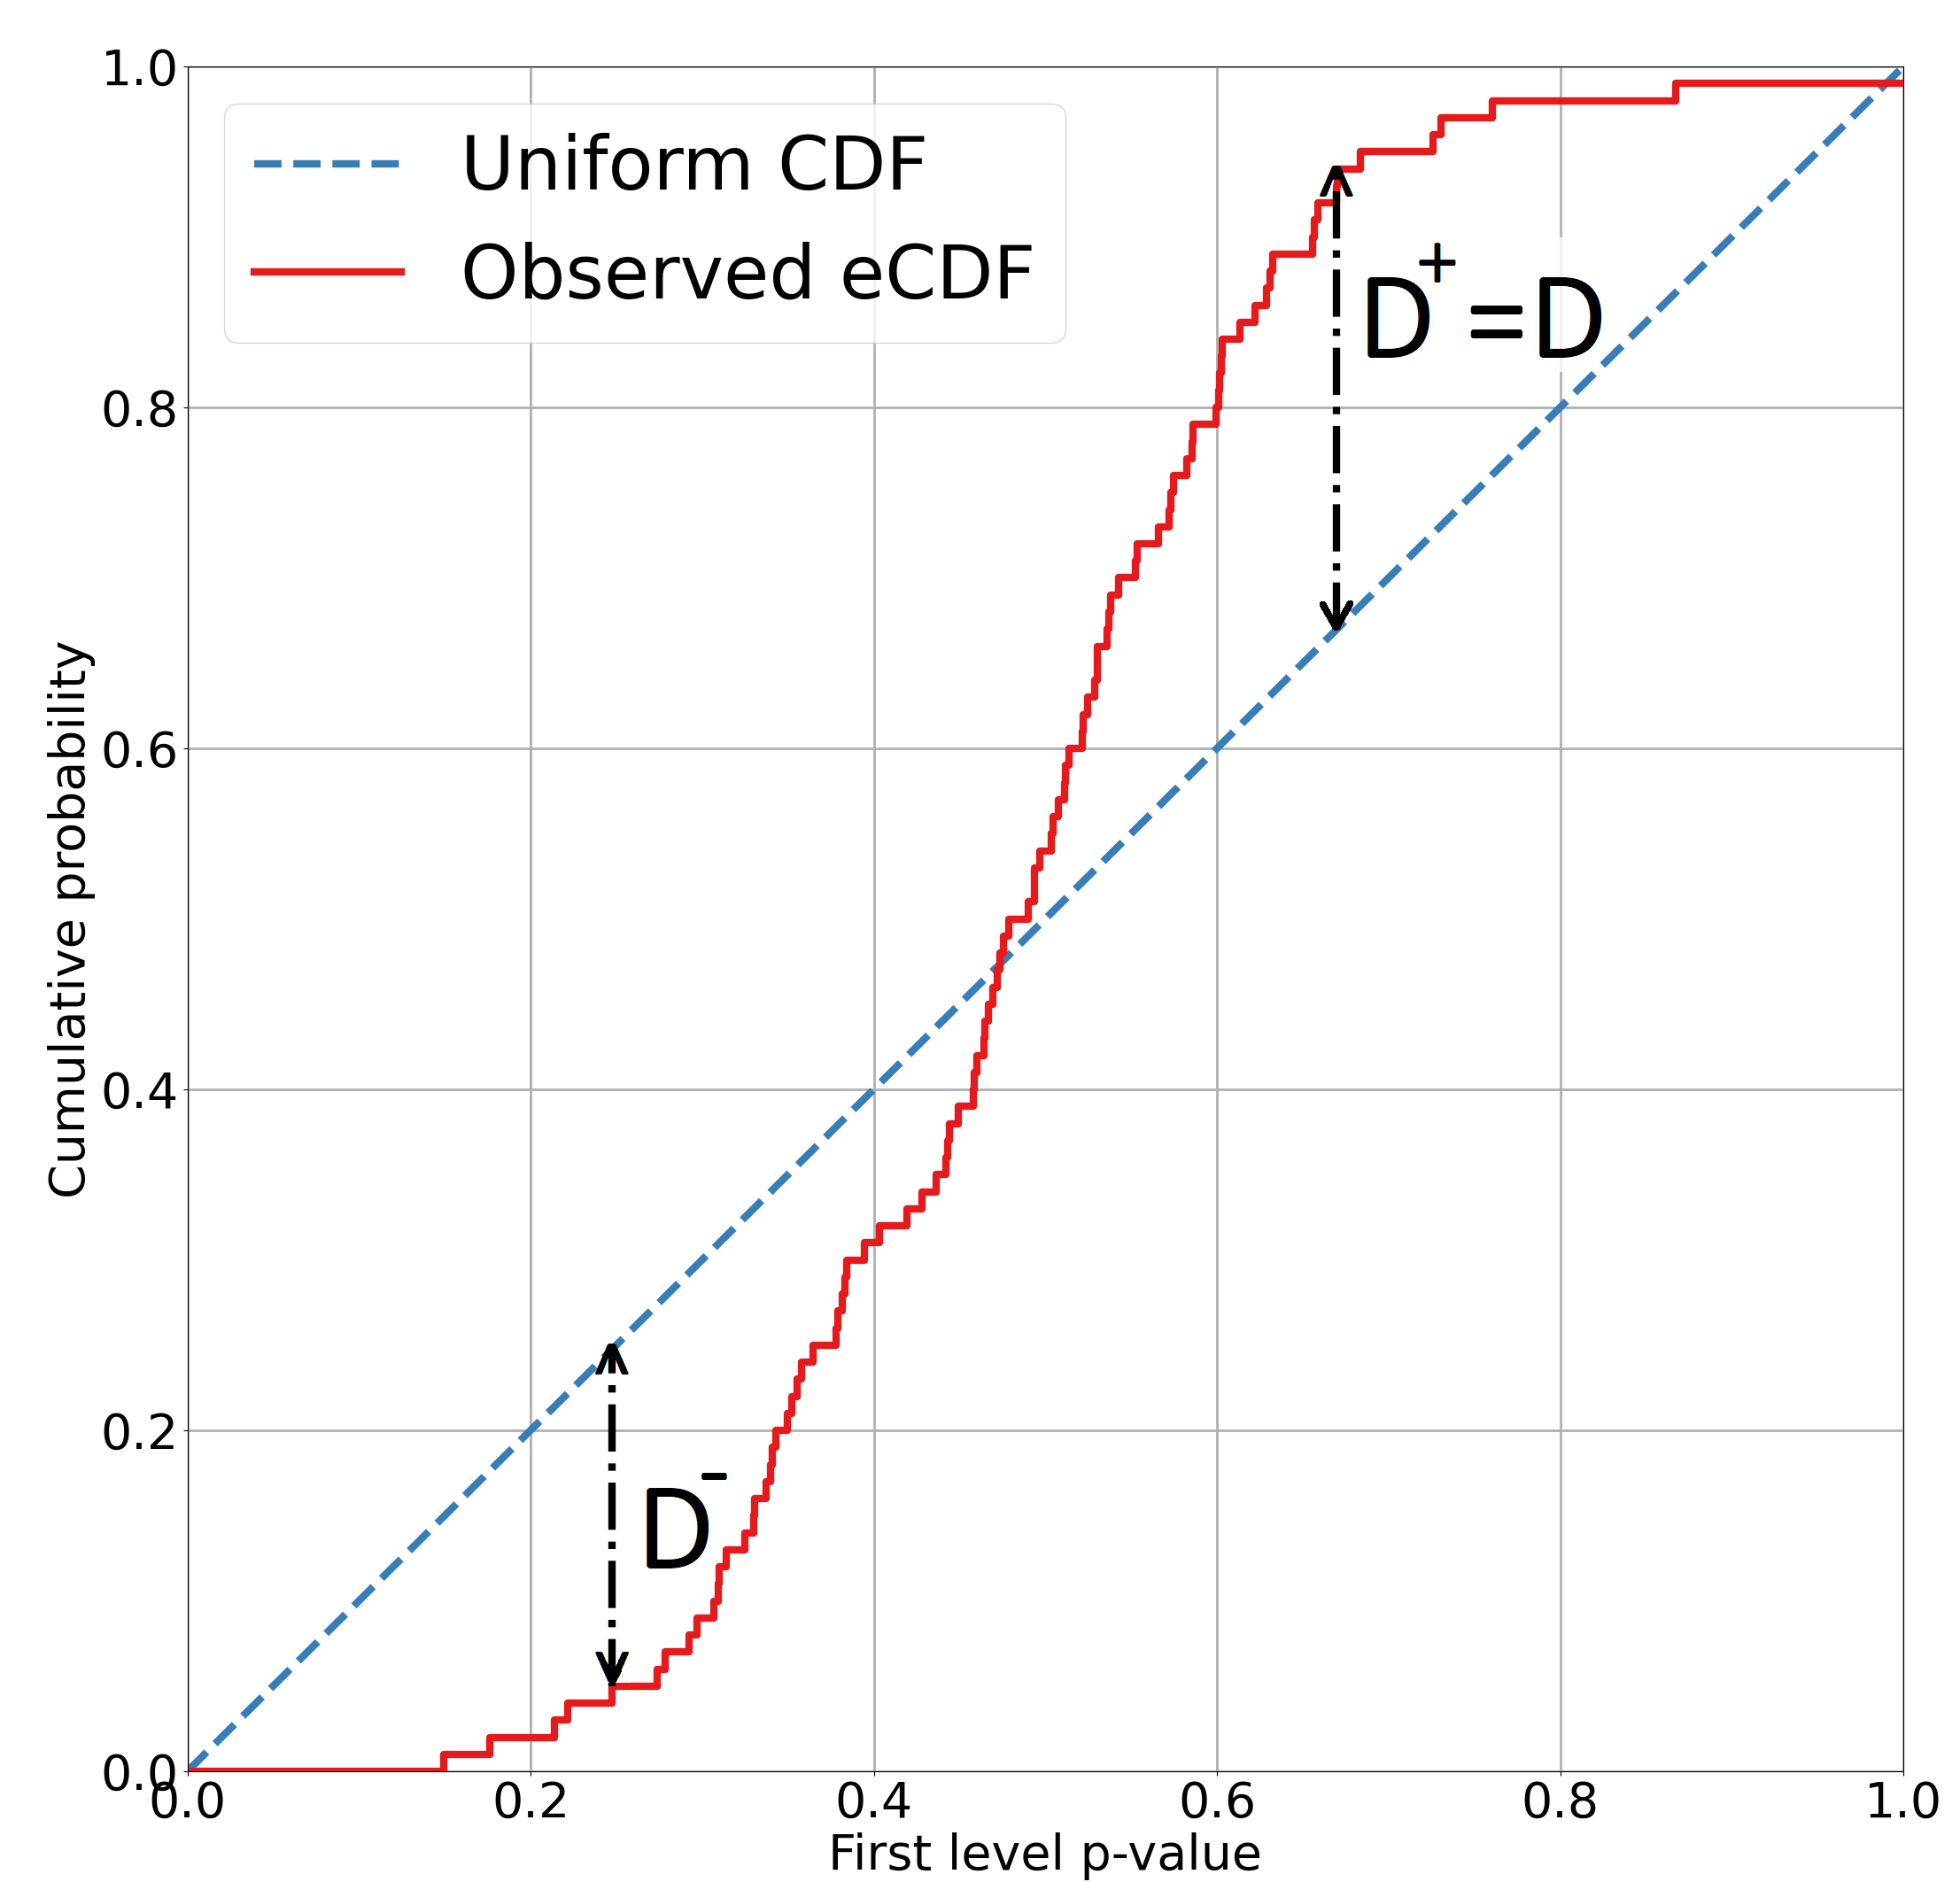
\includegraphics[width=9cm]{figures/ks_d.png}
  \end{center}
  \caption{Visualization of Kolmogorov-Smirnov test statistics for expected uniform distribution and observed data sample.}
  \label{fig:ks_d}
\end{figure}

% $\chi^2$ description (GOF - 100)
\subsection{Chi-squared test}

The Pearson's $\chi^2$ test is used to find statistically significant difference between frequencies of categories in two sets of categorical data. The first-level p-values are split into $k$ equal-width bins (categories) and their respective frequencies are counted. The counted frequencies are compared to the expected frequencies.

For data with $k$ categories the test statistic $\chi^2$ is defined as \[\chi^2 = \sum_{i=1}^{k} \dfrac{(x_i - m_i)^2}{m_i} \]
where $x_i$ is the observed frequency in $i$-th category and $m_i$ is the expected frequency in $i$-th category. For first-level p-values, the expected frequency is equal in each interval. For a correct test the expected frequency in each category must be at least five. \cite[p. 171]{stat-procedures}

% Two-level example
\subsection{Example}

In the two-level test example, I will test one sequence using both one and two-level tests to demonstrate the difference between them. First, the sequence is tested using the one-level Frequency (Monobit) test from NIST STS battery.\cite[p. 2-2]{nist_special} Then the same sequence is assessed by the two-level test using the Frequency test as the first-level test and KS and $\chi^2$ tests as second-level test. Let
\[\begin{split}
    \epsilon =\:15\: &* (100\:consecutitive\:zeroes) + \\
    15\:&*\:(100\:alternating\:ones\:and\:zeroes) + \\
    5\:&*\:(55\:zeroes\:and\:45\:ones)\:+\:\\
    15\:&*\:(100\:consecutive\:ones)
\end{split}\]
be the tested sequence. 

Result of the one-level Frequency test for the sequence $\epsilon$ is p-value $\approx$ 0.479. The null hypothesis is accepted for both $\alpha = 0.01$ and $\alpha = 0.05$ and the sequence $\epsilon$ is considered random. This sequence however clearly contains a pattern, therefore the probability of it being generated by a perfect random number generator is very low.

For the two-level test, the sequence $\epsilon$ is split into $n=50$  disjoint 100 bit long subseqeunces. The Monobit test is applied on each subsequence resulting in set of first-level p-values shown in Table \ref{tab:first_pvalues}.

\begin{table}
  \begin{tabularx}{0.4\textwidth}{ll}
    \toprule
    p-value & occurrences  \\
    \midrule
    $1.52 \cdot 10^{-23}$ & $30$\\
    $0.31$ & $5$\\
    $1.0$ & $15$\\
    \bottomrule
  \end{tabularx}
  \caption{First-level p-values produced by Monobit test}
  \label{tab:first_pvalues}
\end{table}

Last step is to apply the goodness-of-fit tests. The first applied test is the Pearson's $\chi^2$ test with $k=10$ (number of categories), the expected frequency of p-values in each category is five. The statistic of the test is
\[\chi^2 = \sum_{i=1}^{10} \dfrac{(x_i - 5)^2}{5} = 180 \]
and the p-value of this test is $p\approx5.06\cdot10^{-34}$. The null hypothesis is rejected for both $\alpha = 0.01$ and $\alpha = 0.05$. 

Next, the Kolmogorov-Smirnov test is applied. The eCDF is calculated and then the D statistic is computed. The statistic is $D = 0.6$ and results in p-value $\approx 9.63\cdot10^{-18}$. Again, the null-hypothesis is rejected for both $\alpha = 0.01$ and $\alpha = 0.05$ and the sequence is considered non-random.

\begin{figure}
  \begin{center}
    %% minimus is about 100 pixels per 1 centimeter or 300 pixels per 1 inch.
    %% The optimum is about 250 pixels per 1 centimeter 
    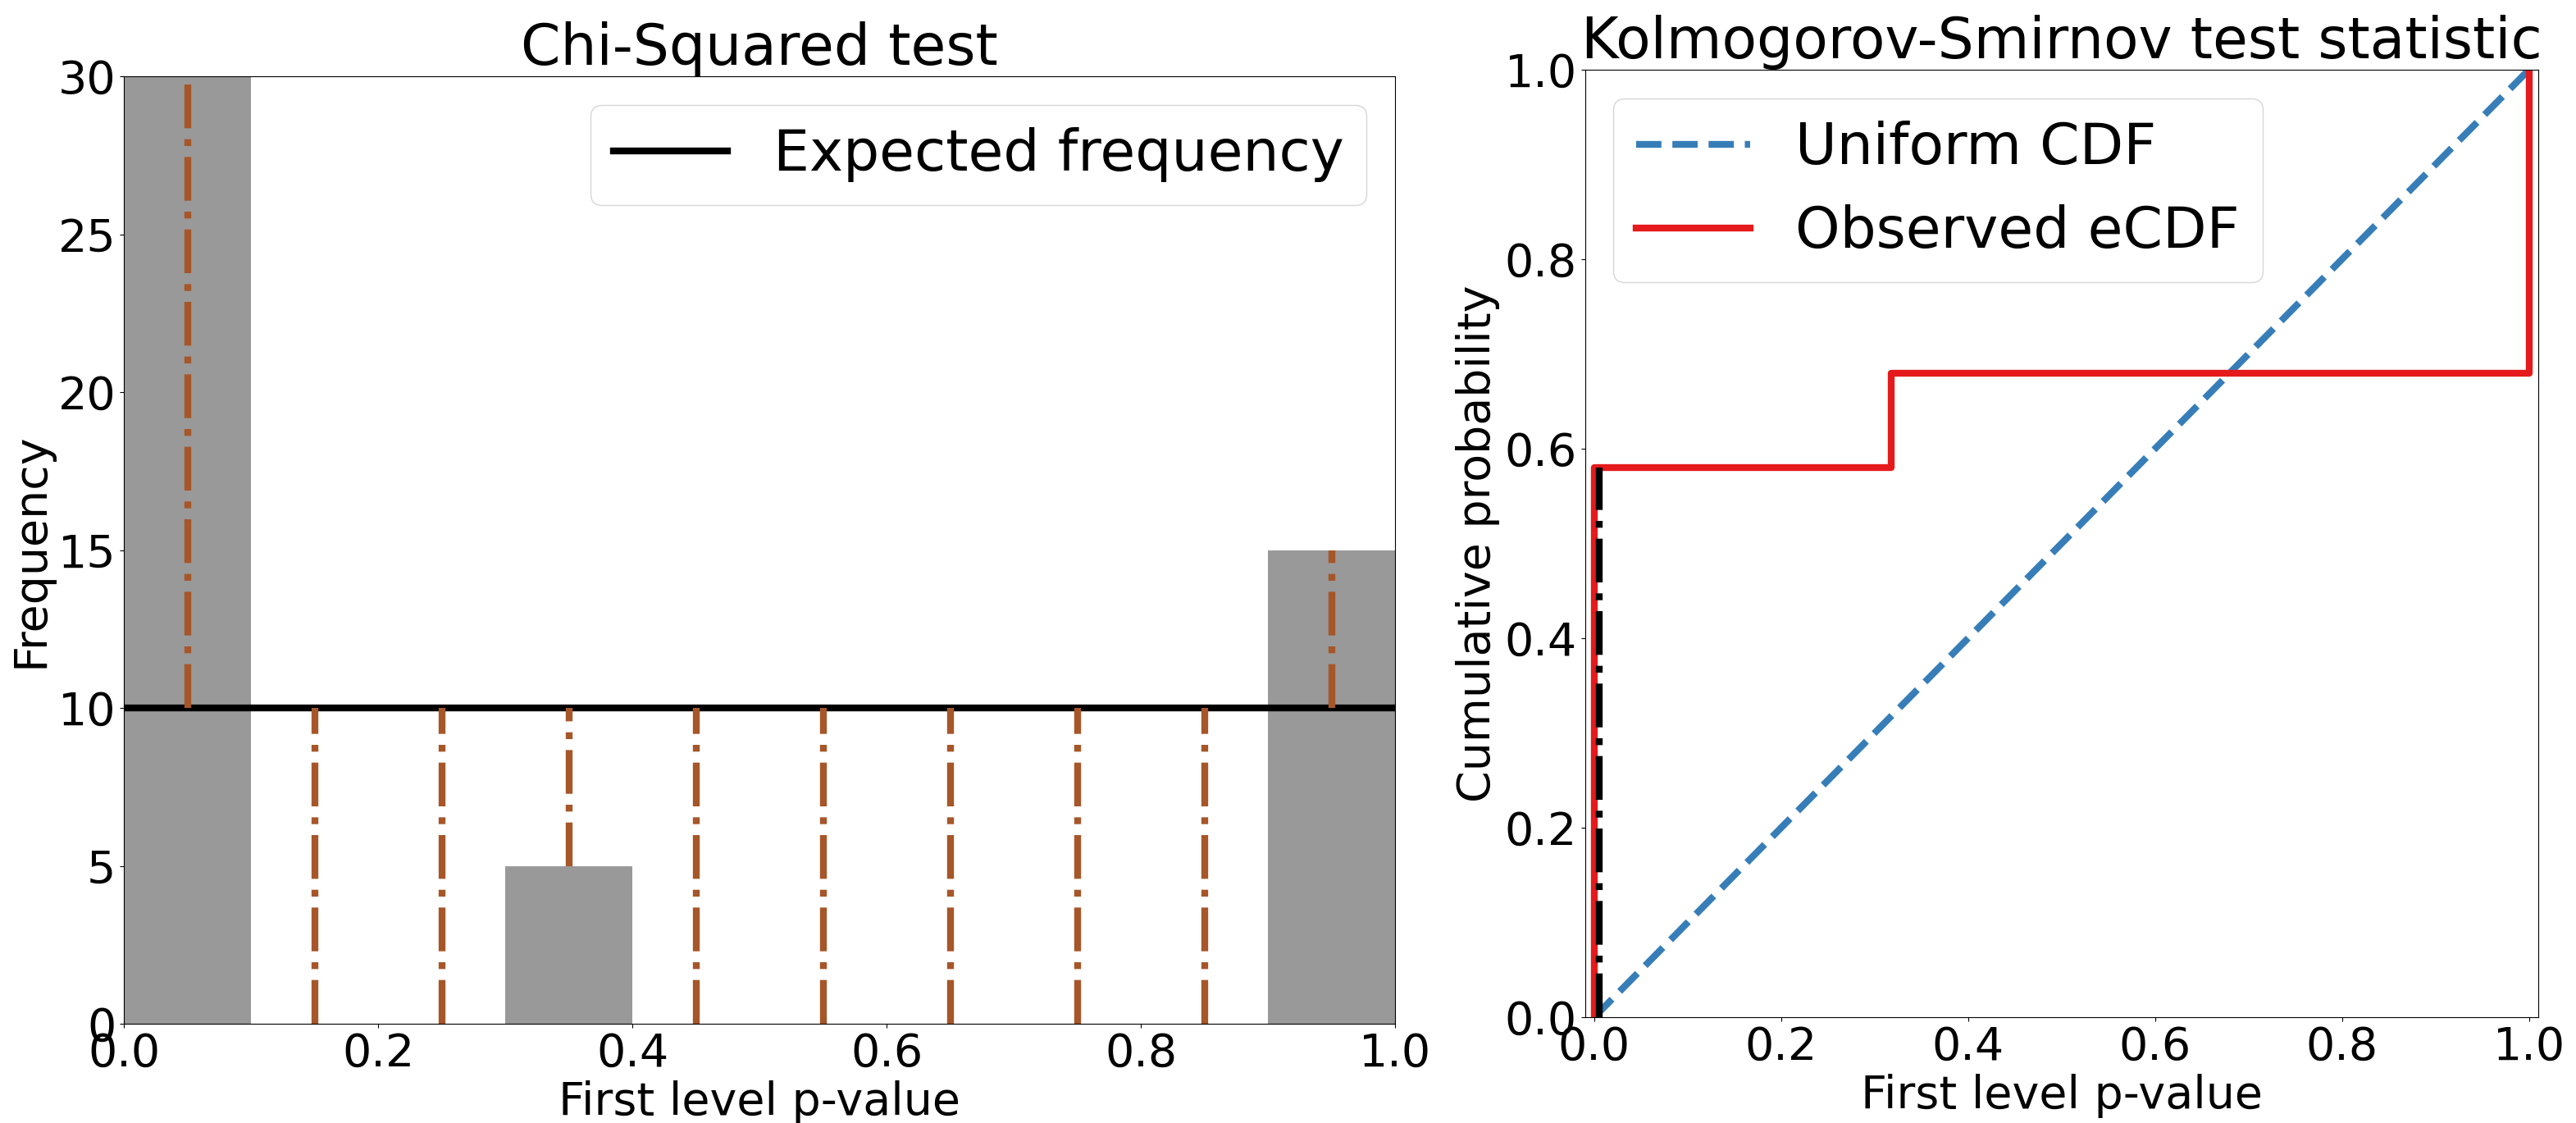
\includegraphics[width=12.5cm]{figures/two_example.png}
  \end{center}
  \caption{Visualisations for $\chi^2$ and KS tests for two-level test example.}
  \label{fig:two_example}
\end{figure}

%%%%%%%%%%%%%%%%%%%%%
%AVAILABLE SOLUTIONS
%%%%%%%%%%%%%%%%%%%%%

\chapter{Programms for randomness tesing}
In this chapter, available programms for randomness testing are presented. In the first section, \emph{statistical testing batteries} (later referred to only as batteries) are described. The second section shows \emph{randomness testing toolkits}, which encompass several batteries together. For both batteries and testing toolkits, overview of setup and output is given.

\section{Statistical testing batteries} \label{chap:sols-batteries}
%battery, individual test - mapping to test statistic
%Mention overflow detection
%If there are any problems with the battery (e.g. tests which read different amount of data from DieHarder). -
%how batteries interpret results (first/second level, more statistics)
%strong and weak things 
%describe output / image
%General description of battery - set of tests, choose test by ID, set tested file \\
%individual test - smallest executable part, possibly more test statistics, setting of the test(ntup, bitw...), data consumption (fixed vs set by user), number of first levels, return-first level pvalues, second-level p-value,


% (Obratil 2, tu01 guide 5)

\emph{Statistical testing battery (suite)} is a set of randomness tests with predefined parameters that allows the user to conveniently apply randomness tests. \cite[p. 5]{tu01_guide} Because all of the batteries share significant similarities, an \emph{abstract battery} is presented to demonstrate the principles. Then, each battery is presented in more detail, mapping its features to the \emph{abstract battery}.

% TODO: data consumption of tests
The \emph{abstract battery} consist of $n$ individual tests, which are distinguished by \emph{test IDs}. Usually one individual test maps to one two-level test. Some individual tests consist of more \emph{subtests}. 

Each \emph{subtest} maps to one two-level test When executing an individual test, all its subtests are executed. The test statistics of subtests are usually related to each other by using the same operation on the tested sequence. For example, the Diehard Craps Test plays 200~000 games of craps. The two calculated first-level test statistics are based on number of wins and GOF test of distribution of throws needed to end the game. \cite{dieharder_orig}

\emph{Variant of the test} is individual test that is parametrized to search for modified pattern in the data. Only some of the individual tests allow such parametrization. Usually, all possible \emph{variants} of given individual test are executed.  \cite[p. 2]{vavercak}

Usually, the following settings are required for each \emph{individual test}. They can be set either \emph{globally} with same values for all tests, or \emph{individually}:
\begin{markdown*}{%
  hybrid,
  definitionLists,
  footnotes,
  inlineFootnotes,
  hashEnumerators,
  fencedCode,
  citations,
  citationNbsps,
  pipeTables,
  tableCaptions,
}

* \emph{number of first-level tests} - Sets how many times the first-level test is repeated (i.e. how many first-level p-values will be produced).
* \emph{size of first-level subsequence} - Sets how long are the subsequences used for first-level test.
* \emph{choose variant} (if applicable for given test).


\end{markdown*}



%(Obratil 3), cite rewind problem (maybe rtt git?)
Originally, the testing batteries were designed to test the random number generators by taking data directly from them as needed. However, common way to test RNG is to take a sample of output, store it into a file and then test contents of the file. The tested file is rewound to the beginning before each individual test (all tests are executed over the same sequence). When the generator is tested directly, every test is executed on 'fresh' sequence. 

Testing files leads to need of \emph{file rewind} detection. File rewind occurs when the tested file is not large enough for given test configuration. In this case, some parts of the file are tested twice during one test and the results may be biased. The needed data size is calculated as \emph{number of first-level tests} $\cdot$ \emph{size of first-level sequence} and it is up to the user to prevent \emph{file rewinds} by configurings the batteries.

%Because unlike random number generators files have limited data size, it is up to user to set the tests to not need more data than are available in the file. Otherwise, when all data from the file have been read but the test needs more, the file is rewound back to the beginning and read again. In such case, the test results might be biased and misleading. The needed data size is calculated as \emph{number of first-level tests} $\cdot$ \emph{size of first-level sequence}.

\subsection{Dieharder} \label{chap:sols-dieharder}
%Explain p-samples, name tests with irregular read bytes, tsample
The \emph{Dieharder} battery was developed as an extension to an older \emph{Diehard} battery. The \emph{Dieharder} is available from \cite{dieharder_orig} or as package in some Unix distributions. Both \emph{RTT} and \emph{rtt-py} use a version of \emph{Dieharder} with modified output format available from \cite{rtt-batteries}.

31 individual tests are contained in the Dieharder. However, four of them are marked as 'Suspect' or 'Do Not Use' and should not be used. Test variants are possible in four tests.

The \emph{Dieharder} allows all settings as described in the \emph{abstract battery}. They are:
\begin{markdown*}{%
  hybrid,
  definitionLists,
  footnotes,
  inlineFootnotes,
  hashEnumerators,
  fencedCode,
  citations,
  citationNbsps,
  pipeTables,
  tableCaptions,
}
* \emph{psamples} argument sets the number of first-level tests. Default value is 100.
* \emph{tsamples} arguments sets the length of first-level subsequences. Units are \emph{random entities}, which are different size for each test. The tests have various default values, some tests ignore this argument.
* \emph{ntup} argument chooses \emph{test variant} for relevant individual tests.

\end{markdown*}
% add KS test computation
%Second-level test employed in Dieharder is the Kolmogorov-Smirnov test. Assessment of the result is done by the battery resulting is PASSED, WEAK or FAILED. The default value of \emph{significance level} is $\alpha=0.000001$.

% result table description
Results of the \emph{Dieharder} are printed to standard output in a table of results. Each row of the table contains results of one individual test or subtest. Columns contain \emph{test name}, value of \emph{ntup} argument (if applicable, usually 0 otherwise), \emph{tsample} and \emph{psamples} values. Last two columns are the \emph{second-level p-value} and \emph{assessment}. Dieharder output can be modified using \emph{output flags}, including the possibility to print all first-level p-values. Example of Dieharder output can be found in Appendix \ref{append:dieharder-output}.

The \emph{file rewinds} are detected by Dieharder automatically. In such case message '\texttt{\# The file file\textunderscore input\textunderscore raw was rewound <n> times}' is printed to error output. Alternatively, by using dedicated output flag, the amount of data used and this message are printed to standard output after each individual test.

\subsection{NIST STS} \label{chap:sols-nist}
% Second-level p-value x^2, 10 categories (nist_special 4-2)

% NIST overview
Original NIST STS\footnote{National Institute of Standards and Technology - Statistical Test Suite} implementation is available from \cite{nist_site}. Optimized version developed by CRoCS FI MU \cite{nist_special} is used in RTT, available from \cite{rtt-batteries} \emph{NIST STS} contains 15 individual tests with no variants. Allowed settings are:
\begin{markdown*}{%
  hybrid,
  definitionLists,
  footnotes,
  inlineFootnotes,
  hashEnumerators,
  fencedCode,
  citations,
  citationNbsps,
  pipeTables,
  tableCaptions,
}
* \emph{Stream count} argument denotes the number of first-level tests and must be set by the user. For a statistically meaningful result of second-level test should be at least 55. 
* \emph{Stream size} argument sets the length of first-level subsequences in \emph{bits} and must be set by the user. The tests have various recommendations for minimal size.
\end{markdown*}

The second-level p-value is computed using the $\chi^2$ test after dividing the first-level p-values into $k=10$ categories. The NIST STS also calculates the proportion of subsequences passing the first-level test. \cite[p. 4-1]{nist_special}.

Tests results are stored in files inside \emph{experiments/AlgorithmTesting} folder. Table with overview of results is in file \emph{finalAnalysisReport.txt}. Each row contains one individual test or subtest. First 10 columns are observed frequencies of first-level p-values in given category. The \emph{second-level p-value, proportion of subsequences passing the first-level test} and \emph{test name} follow. 

More results information for each test are stored in corresponding folders. In file \emph{stats.txt} the first-level p-values, test statistics and other computational information are stored. In file \emph{results.txt}, only the first level p-values are stored. Example of output is available in Appendix \ref{append:nist-output}.

The file rewind is detected automatically by the battery. In such case, message '\texttt{READ ERROR:  Insufficient data in file.}' is printed to standard output.


\subsection{Test U01} \label{chap:sols-testu01}
%TODO: no second level assessment
%TODO: output format

TestU01 was developed to be a state-of-the-art software library oriented on testing of random number generators and is available from \cite{tu01_site}. It contains several batteries, used in \emph{RTT} and \emph{rtt-py} are the \emph{SmallCrush, Crush, BigCrush, Rabbit, Alphabit} and \emph{BlockAlphabit}. Because TestU01 is a software library only, custom command-line interface was created for use in RTT (also used in \emph{rtt-py}), available from \cite{rtt-batteries}. The TestU01 does not apply a two-level test, it only allows to repeat the single-level test. In this battery, the \emph{individual test} maps to the repeated \emph{single-level test}. If the user wishes to apply the second-level test, they have to examine the distribution of single-level tests on their own.

Each battery in TestU01 allows for a different set of user settings. All possible arguments in TestU01 are:
\begin{markdown*}{%
  hybrid,
  definitionLists,
  footnotes,
  inlineFootnotes,
  hashEnumerators,
  fencedCode,
  citations,
  citationNbsps,
  pipeTables,
  tableCaptions,
}

* \emph{repetitions} argument sets how many times the single-level test is executed
* \emph{bit\textunderscore nb} argument sets the length of first-level subsequences in \emph{bits}. Applicable (and mandatory) only for Rabbit, Alphabit and BlockAlphabit.
* \emph{bit\textunderscore w} argument is used to choose test variant. Only in \emph{BlockAlphabit} battery.
\end{markdown*}
Unlike other batteries, the TestU01 batteries do not employ the \emph{second-level test}. The assessment  of first-level p-values uniformity is up to the user. 

% output format
The output format is same of for all of TestU01 batteries and is printed to standard output. Only one individual test is executed during one battery run, for which the following is printed. For each repetition of single-level test the test name and all test parameters are printed. Then the test static value and its corresponding p-value is printed (or more values, if the individual test contains subtests). After each single-level test, a \emph{generator state} is printed, containing information about how many data were used in all first-level tests so far. And the end of the individual test report, list of all p-values is printed. Example output is in Appendix \ref{append:tu01-output}.

% overflow detection - reading 10MB blocks
File rewind detection is done partially by the batteries using the \emph{generator state} information, however it is up to the user to interpret it. The \emph{generator state} contains three fiels - \emph{bytes need for testing} (number of bytes that were indeed used for testing), \emph{bytes read from file} (number of bytes that were read from tested file) and \emph{total number of file rewinds}. 

Because the data are read from file in 10MB long blocks, the number of file rewinds may be positive, but the number of \emph{bytes needed for testing} will be lower than the actual file size, causing a false alarm. It is up to the user to manually check this situation. % TODO check crush family error detection


%crush family
\subsubsection{SmallCrush, Crush, BigCrush}
Batteries from the \emph{Crush} family were created to test general use random number generators. The batteries contain 10, 96 and 106 tests with increasing demand for data size and runtime. The intended use is to apply SmallCrush for a quick assessment. If the the sequence is accepted, more stringent Crush and BigCrush batteries are applied. The size of first-level sequence cannot be changed. \cite[p. 242]{tu01_guide}

%rabbit
\subsubsection{Rabbit}
The Rabbit battery contains 26 individual tests. The \emph{bit\textunderscore nb} argument must be set by the user to a value of at least 500. \emph{At most} \emph{bit\textunderscore nb} will be used for first-level subsequence size. \cite[p. 152]{tu01_guide} However, several tests require significantly longer subseqeunce than 500 bits. Some tests use significantly shorter subsequence than specified by \emph{bit\textunderscore nb}.

\subsubsection{Alphabit and BlockAlphabit}
Both Alphabit and BlockAlphabit batteries contain the same nine individual test. In the BlockAlphabit battery, the tested data are transformed to deploy \emph{test variants}. The test variant is chosen by the \emph{bit\textunderscore w} argument parametrizing the transformation, which takes values from set \{1, 2, 4, 8, 16, 32\}. \cite[p. 155]{tu01_guide} Size of the first-level sequences will be \emph{at most} the size set by \emph{bit\textunderscore nb} argument.


% FIPS
\subsection{FIPS Battery} \label{chap:sols-fips}
The FIPS\footnote{Federal Information Processing Standards} battery contains five tests and is based on FIPS 140-2 standard. Custom command-line interface of the battery was created for \emph{rtt-py} available from \cite{rtt-py-batteries}. The interface is based on implementation taken from \cite{fips-site}. No test variants are available and the length of first-level sequence is set to 2500 bytes and cannot be changed \cite[p. 20]{vavercak}. Only one arguments is available:
\begin{markdown*}{%
  hybrid,
  definitionLists,
  footnotes,
  inlineFootnotes,
  hashEnumerators,
  fencedCode,
  citations,
  citationNbsps,
  pipeTables,
  tableCaptions,
}
* \emph{bytes count} argument sets how many bytes will be used for testing \emph{altogether}, determining the \emph{number of first-level tests} %$\lfloor bytes\textunderscore~count~\div~2500\rfloor$ .
\end{markdown*}

Output of FIPS battery is printed to standard output and in user-specified file in JSON\footnote{JavaScript Object Notation} format. First, information about accepting or rejecting the null-hypothesis is printed. Then a list of individual tests results is printed. For each individual test, the test name, number of failures and number of runs is printed. Example output is in Appendix \ref{append:fips-output}

File rewinds are detected automatically by the battery. In such case, the battery will not run and will print message '\texttt{Error (<filename>) ! File is not big enough}' to error output.

% BSI
\subsection{BSI battery} \label{chap:sols-bsi}
The BSI\footnote{Bundesamt für Sicherheit in der Informationstechnik} battery contains nine test and is based on series of standards released by BSI. \cite[p. 3]{vavercak} For use in \emph{rtt-py} a custom command-line interface was created, available from \cite{rtt-py-batteries}. The tests implementations were extracted from the ParanoYa application. \cite[p. 16]{vavercak}

No test variants are available in the BSI battery. Each test has its own preset \emph{first-level subsequence size}, which cannot be changed. One argument is available for the battery:
\begin{markdown*}{%
  hybrid,
  definitionLists,
  footnotes,
  inlineFootnotes,
  hashEnumerators,
  fencedCode,
  citations,
  citationNbsps,
  pipeTables,
  tableCaptions,
}
* \emph{bytes count} argument sets how many bytes will be read from the tested file. The number of \emph{first-level tests} is calculated based on this value.
\end{markdown*}

Output of BSI battery is printed to standard output and in user-specified file in JSON format. It contains list of individual tests results. For each individual test, a name and information whether \emph{total error} occurred is printed. If no \emph{total error} occurred, number of failures and number of runs is printed as well. Example output is available in Appendix \ref{append:bsi-output}.

File rewinds are detected automatically by the battery. In such case, the battery will not run and will print message 
'\texttt{File is not big enough}' to error output.



% testing toolkit
\section{Testing toolkits}\label{chap:sols-toolkits}
In the previous section different randomness testing batteries were described. The typical user, however, uses more than one battery, which means installing and running each testing battery individually. Also it is strongly recommended (sometimes even needed) to set up parameters for each test from the battery individually based on size of the tested file and to run this test manually.

Since this approach is not convenient, Center for Research on Cryptography and Security (CRoCS) at FI MU created the Randomness Testing Toolkit (\emph{RTT}).\cite{obratil} This toolkit allows users to run and configure eight test batteries using the same command.

This work was followed by Patrik Vaverčák from Faculty of Electrical Engineering and Information Technology at Slovak University of Technology. He created newer variant of \emph{RTT} called Randomness Testing Toolkit in Python (\emph{rtt-py}). \cite{vavercak}

% RTT OLD
\subsection{Randomness Testing Toolkit} \label{chap:sols-rtt}

\emph{RTT} was created in 2017 and its main idea was to combine \emph{Dieharder}, \emph{NIST STS} and all batteries from \emph{TestU01} mentioned in Subection \ref{chap:sols-testu01} into one program. It was written in C++. The concept is that \emph{RTT} acts only as a unified interface of the batteries. Each test battery is executed by \emph{RTT} as a separate program. The \emph{RTT} then collects the output and processes it into a unified format.~\cite[p.~8]{rtt-obratil}

RTT is available from CRoCS GitHub repository \cite{rtt-site}. All of the batteries used in RTT are available from a single GitHub repository \cite{rtt-batteries}. Before running, user has to install both the \emph{RTT} and used batteries as described GitHub project wiki. If the user intends to run NIST STS, the \emph{experiments} folder has to be moved (or linked) to \emph{working directory} of RTT. This is not noted anywhere.

\subsubsection{RTT settings}\label{rtt-settings} 
The \emph{RTT} needs to be set up by the user before running. The first part of user settings contains \emph{general settings} of the \emph{RTT}, the second part contains individual \emph{batteries configurations}. Each of these parts is stored in its own JSON file. 

The \emph{general settings} are stored in \emph{rtt-settings.json} file, which is located in the working directory of the \emph{RTT}~\cite[p.~10]{rtt-obratil}. These settings are not expected to change. The most important setting from the general part are paths to the executable binaries of individual statistical test batteries. This is the only setting that has to be manually filled in by the user.

The storage database can also be filled in by the user, but this functionality optional. The following general settings have implicit values and do no need to be changed unless the user wishes to. They are paths to storage directories for results and logs of individual runs and execution options (test timeout and maximal number of parallel executions of tests). 

The battery configurations are dependant on the size of the tested file, therefore the file with the battery configuration is specified for each run of the \emph{RTT} as one of its arguments. These configurations are different for each battery (see Section \ref{chap:sols-batteries}), but they all follow the same format and are stored together in a single file.~\cite[p.~11]{rtt-obratil} The \emph{RTT} contains several prepared battery configurations for various sizes of tested file.

For each battery, the settings are split into two parts - \emph{defaults} and \emph{test-specific-settings}. The \emph{defualts} section contains IDs of individual tests to be run and default values of all arguments. The \emph{test-specific-settings} is a list of all tests whose settings are different than those in \emph{defaults} (along with new settings) or tests which employ test variants. In the second case, all variants to run are listed in entry for the given individual test.

\subsubsection{RTT output}
The output of \emph{RTT} is in a plain text format. The most important part of the output is the direct report, which is saved in the \emph{results} directory. At the beginning of the report are general information -- the name of the tested file, the name of the used battery, ratio of passed and failed individual tests and battery errors and warnings in case there were any.

% terminology - single x individual test
After the general information is a list of results of individual tests in a unified format. The fist part of the individual test report contains the name of the test and user settings. The second part of the single test report are the second-level p-values alongside the names of statistic used (usually Kolmogorov-Smirnov or $\chi^2$ statistic). At the end of the single test report is a list of first-level p-values produced by the test. Example of the output can be seen in Figure \ref{fig:rtt_output_example}.

\begin{figure}
  \begin{center}
    %% minimus is about 100 pixels per 1 centimeter or 300 pixels per 1 inch.
    %% The optimum is about 250 pixels per 1 centimeter 
    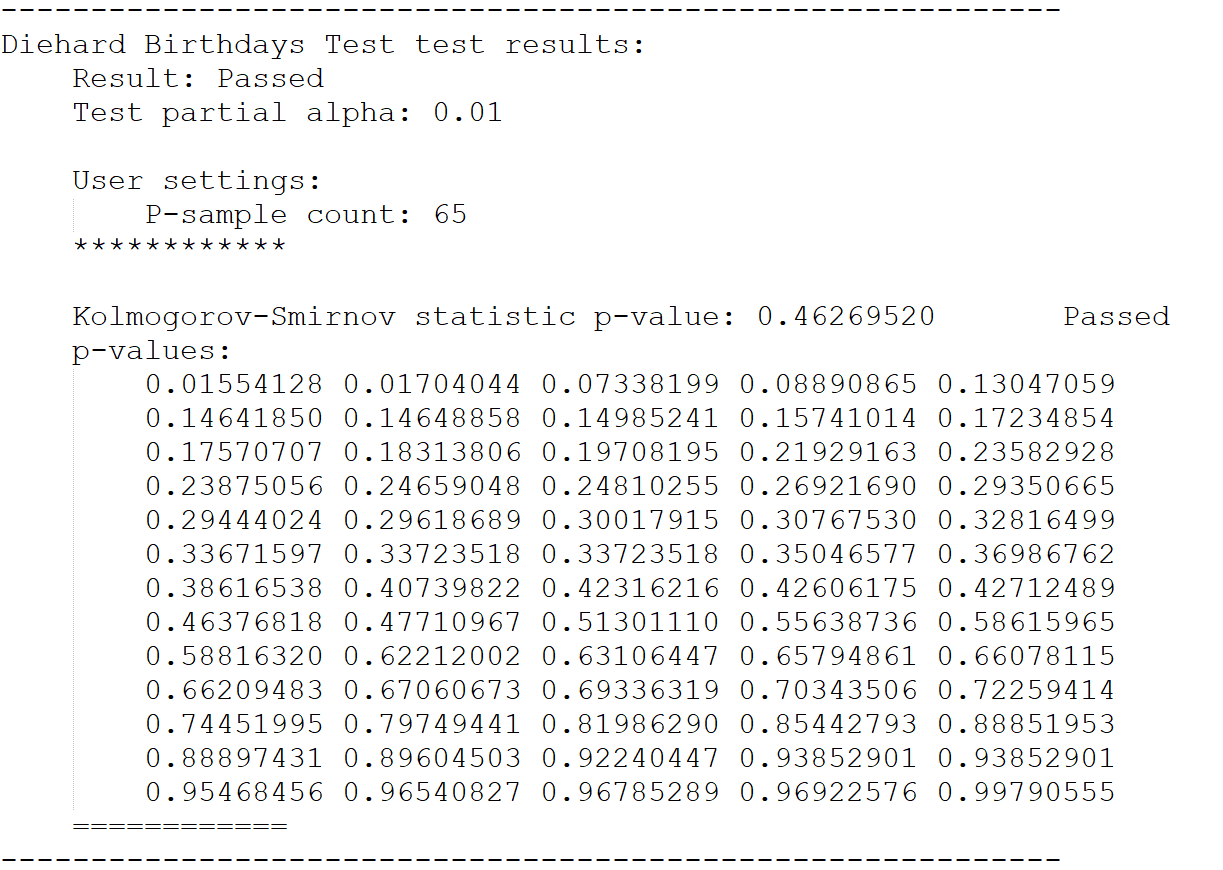
\includegraphics[width=12cm]{figures/rtt_dieharder_output.png}
  \end{center}
  \caption{The example of single test report from the \emph{RTT}}
  \label{fig:rtt_output_example}
\end{figure}

%\subsection{Disadvantages}
%The problems/weak points we want to improve with this thesis. Namely at least non machine-machine readable format, running only one battery at time, maybe re-calculation of results

%There are two most notable disadvantages of the \emph{RTT}. The first one is that each battery has to be run individually by the user. This lowers the convenience of usage for the user. The second one is the output format. While it is easy to read for human users, machine reading requires complicated parsing. 


\subsection{Randomness Testing Toolking in Python} \label{chap:sols-rtt-py}
The Randomness Testing Toolkit in Python (\emph{rtt-py}) was created by Patrik Vaverčák. It is supposed to be an improved version of \emph{RTT} sharing the same concept \cite[p.~24]{vavercak} and it was written in Python.

The included batteries are Dieharder, NIST STS, FIPS battery and BSI battery. \emph{Rtt-py} also includes Rabbit, Alphabit and BlockAlphabit batteries from TestU01. The Crush family batteries are not run, even though arguments of \emph{rtt-py} suggest that they are included. The \emph{rtt-py} allows for multiple files to be tested at once.


The \emph{rtt-py} is available from \cite{rtt-py-site} and implementations of all used batteries are available from \cite{rtt-py-batteries}. Before running, both the \emph{rtt-py} and the batteries have to be installed as described in the project's README.



\subsubsection{Rtt-py settings}
The settings of \emph{rtt-py} use similar format as the original \emph{RTT} (as described in Subsection \ref{chap:sols-rtt}). The \emph{general settings} from the \emph{RTT} should be one-way compatible with \emph{rtt-py} \cite[p. 25]{vavercak}. In reality there is a problem with settings for the NIST STS's experiments directory. Also, no database connection is implemented in \emph{rtt-py}, therefore the \emph{mysql-db} attribute is ignored. \cite{rtt-py-site}

The second part of user settings are the battery configurations. They use the same format as in \emph{RTT} (as mentioned in \ref{rtt-settings}) and are interchangeable.~\cite[p.~25]{vavercak} The user has to keep in mind that the \emph{rtt-py} uses FIPS and BSI batteries, which are not used in \emph{RTT}. 

\subsubsection{Rtt-py output}
The \emph{rtt-py} creates output in two formats -- \emph{CSV}\footnote{Comma-separated values} and \emph{HTML}\footnote{Hypertext Markup Language}. \cite[p. 36]{vavercak} Both of these report formats contain overview table. Each row from the table represents results of one individual test or subtest. The first column contains the name of the test and the name of the battery it belongs to. The second column contains \emph{failure rate} - ratio of sequences not passing the first-level test.

Each of the following columns is named after one tested file. The record contains either second-level p-value reported by the test, or number of failed runs -- this depends on the battery. Example of this table can be seen at figure \ref{fig:rtt_py_table}.
\begin{figure}
  \begin{center}
    %% minimus is about 100 pixels per 1 centimeter or 300 pixels per 1 inch.
    %% The optimum is about 250 pixels per 1 centimeter 
    \frame{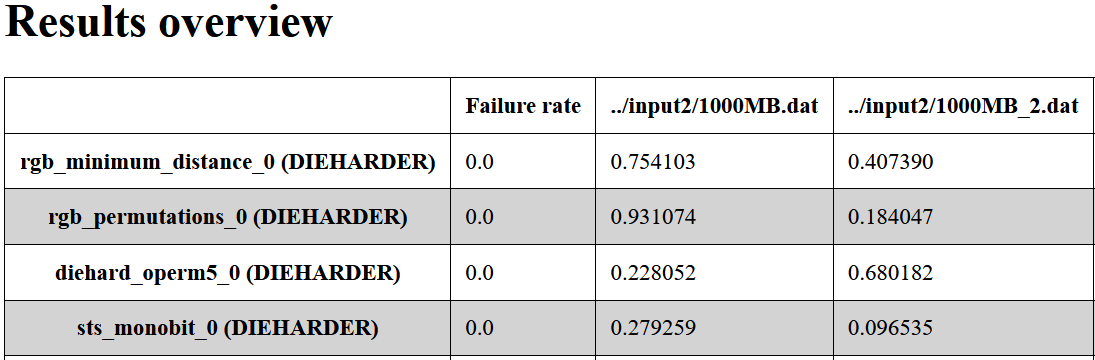
\includegraphics[width=14cm]{figures/rtt-py-table2.png}}
  \end{center}
  \caption{The example of the overview table from the \emph{rtt-py}}
  \label{fig:rtt_py_table}
\end{figure}


The output in the HTML format contains than the output in the CSV format. For each battery and for each tested file an HTML file with reports is generated.

In each report file there is a list of reports for each individual test or subtest from the given battery containing the result (either reported p-value, or number of failed runs). It may contain additional information such as settings of the test or other information connected to the result, depending on the battery and on the executed test. Example of the  report can be seen in figure \ref{fig:rtt_py_html}
\begin{figure}
  \begin{center}
    %% minimus is about 100 pixels per 1 centimeter or 300 pixels per 1 inch.
    %% The optimum is about 250 pixels per 1 centimeter 
    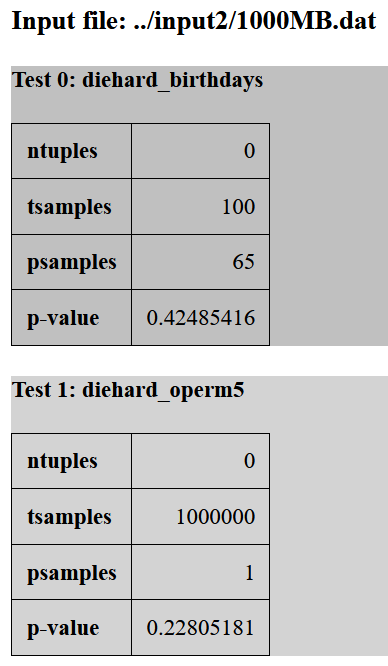
\includegraphics[width=6cm]{figures/rtt-py-dieharder-html.png}
  \end{center}
  \caption{The example of HTML Dieharder report from the \emph{rtt-py}}
  \label{fig:rtt_py_html}
\end{figure}

%\subsection{Disdvantages}
%One of the problems that need to be addressed is that the \emph{rtt-py } ignores errors and warnings from tests. The most notable example why this is a problem is when the tested file does not contain enough data for current battery configuration.

%In this case, the test will read some parts of the data more than once and inform the user about this situation on the error output. The test will still produce result, which will, however, be biased by repeated parts of the tested file.

%This may lead to incorrect interpretation of the results and to false acceptance or false rejection of the tested data. Since the \emph{rtt-py} ignores this, there is no way for the user to be informed about this situation.

%Compared to the \emph{RTT} the reports created by \emph{rtt-py} contain less information. Namely the first-level P-values are ignored, even though they can be useful for deeper examination of the results and the generator.


% TEST ANALYSIS

\chapter{Tests Analysis} 
We can choose from various test statistics. Most of the test statistics in widely used test batteries work with data of fixed length. TODO: REF ANALYSIS CHAPTER However, in some tests data with varying length are tested. These statistics further split into two categories. In the first category, the length of tested data is preset by user. These can be further viewed as fixed-length tests. In the second category, the length of tested data is determined during the testing process.

% DATA CONSUMPTION
\section{Data Consumption} \label{chap:analysis-data}
%several big tables, mention exact parameters the tests  were run with

% configurable x fixed size
% variable x constant

% TODO: fix size for tests
As mentioned in Subsection \ref{chap:sols-batteries}, import part of preventing \emph{file rewinds} is correct configuration of the tests. This is a hard task, because the user has to know size of first-level subsequences. To help with this task, I performed analysis of sizes of first-level subsequences for Dieharder, SmallCrush, Crush, Rabbit, Alphabit and BlockAlphabit batteries.  % TODO why the rest was omitted

% INTRODUCTION
\subsection{Introduction} \label{chap:analysis-data-intro}

The idea was to run all tests from the batteries and calculate how many bytes were used for each individual test or test varint. Based on this information, a table for each battery containing this information was created.

The tests can be split into two cattegories based on users influence on the first-level subseqeunce size. In the subsequent text, I use the following terminology. \emph{Tests with configurable size} are the tests where the size of first-level subsequence can be set by the user. The tests with predefined and unchangable first-level subsequence size are called \emph{tests with fixed size}.

During the analysis another way to split tests into two cattegories was found. This takes into account if all runs of the individual test with \emph{the same settings} have the same first-level subseqeunce size, or if each reads data of different size. The first case is called \emph{tests with constant size}, the second is called \emph{tests with variable size}. 

The size of the first-level subseqeunce in the tests with variable size is based on the \emph{content} of the sequence. TODO: EXAMPLE FROM DIEHARDER. For an \emph{individual} test from this cattegory and for random content of the sequence, the \emph{real} size of the first-level sequence is close to \emph{some} value. Behaviour of the test on \emph{extremely non-random} sequence (for example all zeroes or ones) is different for each test. Some tests read only an extremely small part of the tested data, some tests will cycle.

To examine how long are the first-level sequences of tests with variable size, I run each test from this cattegory at least 100 times on different \emph{random} data (taken from /dev/random). Tests from this cattegory are presented in their own tables. To verify that tests with constant size are indeed constant, I run them several times with different number of first-level sequences.

\subsection{Dieharder}

%args
% "../../../rtt-statistical-batteries-master/dieharder", "-f", input_file, "-S 0 -s 1", "-g 201", "-D 131180","-d {}".format(test_id), "-p 25" if test_id in {13, 16} else "-p 5"
In Dieharder both tests with configurable and fixed size are present. All tests with configurable size have a default setting for first-level sequence size, which is usually used. Therefore all tests from this battery are viewed as tests with fixed size.

\subsection{TestU01 SmallCrush and Crush}
In the SmallCrush and Crush batteries, all tests have fixed size.


% several table, at least table for minims
\subsection{TestU01 Rabbit}
All tests in the Rabbit battery are with configurable size. The size is configured using the \emph{bit\textunderscore nb} argument, where the desired size is entered in \emph{bits} and for use is rounded down to closest multiple of 32. The \emph{bit\textunderscore nb} has no default value, must be at least 500 and \emph{at most} \emph{bit\textunderscore nb} bits will be read from the file. \cite[p. 152]{tu01guide} However, some tests require bigger size of \emph{bit\textunderscore nb} and will not run otherwise. These tests and their required sizes are in Table \ref{tab:analysis_rabbit_minims}. The minims were found and verified experimentally.

\begin{table}
  \begin{tabularx}{0.5\textwidth}{c|c}
    %\toprule
    Test ID & minimal \emph{bit\textunderscore nb}\\
    \midrule
    1& 500\\
    2& 500\\
    3& 500\\
    4& 500\\
    5& 500\\
    6& 500\\
    7& 500\\
    8& 500\\
    9& 31,200\\
    10& 960\\
    11& 960\\
    12& 500\\
    13& 500\\
    14& 500\\
    15& 960\\
    16& 1,920\\
    17& 3,840\\
    18& 500\\
    19& 500\\
    20& 500\\
    21& 51,200\\
    22& 5,120,000\\
    23& 52,428,800\\
    24& 960\\
    25& 30,720\\
    26& 300,480\\
  \end{tabularx}
  \caption{Minimal values of \emph{bit\textunderscore nb} argument needed to run tests from \emph{Rabbit} battery.}
  \label{tab:analysis_rabbit_minims}
\end{table}

Tests 6, 7 and 8 read only data with size $2^k, k \in N$. The possible values of $k$ are different for each test and shown in Table \ref{tab:analysis_rabbit_two_powers}. \cite[p. 124-126]{tu01guide} If the \emph{bit\textunderscore nb} is not power of two, closest lower applicable power of 2 is used. The \emph{bit\textunderscore nb} still has to be at least 500, even though smaller amout of bits may be read.

\begin{table}
  \begin{tabularx}{0.5\textwidth}{c|c}
    %\toprule
    Test ID & maximal $k$\\
    \midrule
    1& 28\\
    2& 20\\
    3& 26\\
 
  \end{tabularx}
  \caption{Maximal values of $k$ for Rabbit tests which take data of size $2^k$ in \emph{bits}.}
  \label{tab:analysis_rabbit_two_powers}
\end{table}

The only test with \emph{variable} size from Rabbit battery is 20. It uses around TODO \% of data size specified by \emph{bit\textunderscore nb} argument. Test 5 

For the following analysis of used first-level subseqeunce sizes the \emph{bit\textunderscore nb} argument was fixed to value 52,428,800.


% Time consumption
\section{Time Consumption} 
again some big tables, choose one test as a reference and the rest will be relative. mention exact parameters, maybe add throughput?
\section{Configuration Calculator}
goal of the config calc, description, usage etc...
\section{P-Values}
Various problems with test p-values distributions, will probably be split into more sections



% IMPLEMENTATIONS COMPARISON
\chapter{Implementations Comparison}

\section{Output}
Mentioned differences\\
for both RTT and rtt-py - subset or whole?

\section{Missing Features of \emph{rtt-py}}

\section{Proposed improvements}
included things: adding first-level p-values, 

% CONCLUSION

\chapter{Conclusion}

%% Start the appendices.
\appendix 

\chapter{Batteries output examples} \label{append:dieharder-output}
\section{Dieharder}

\begin{figure}[h]
  \begin{center}
    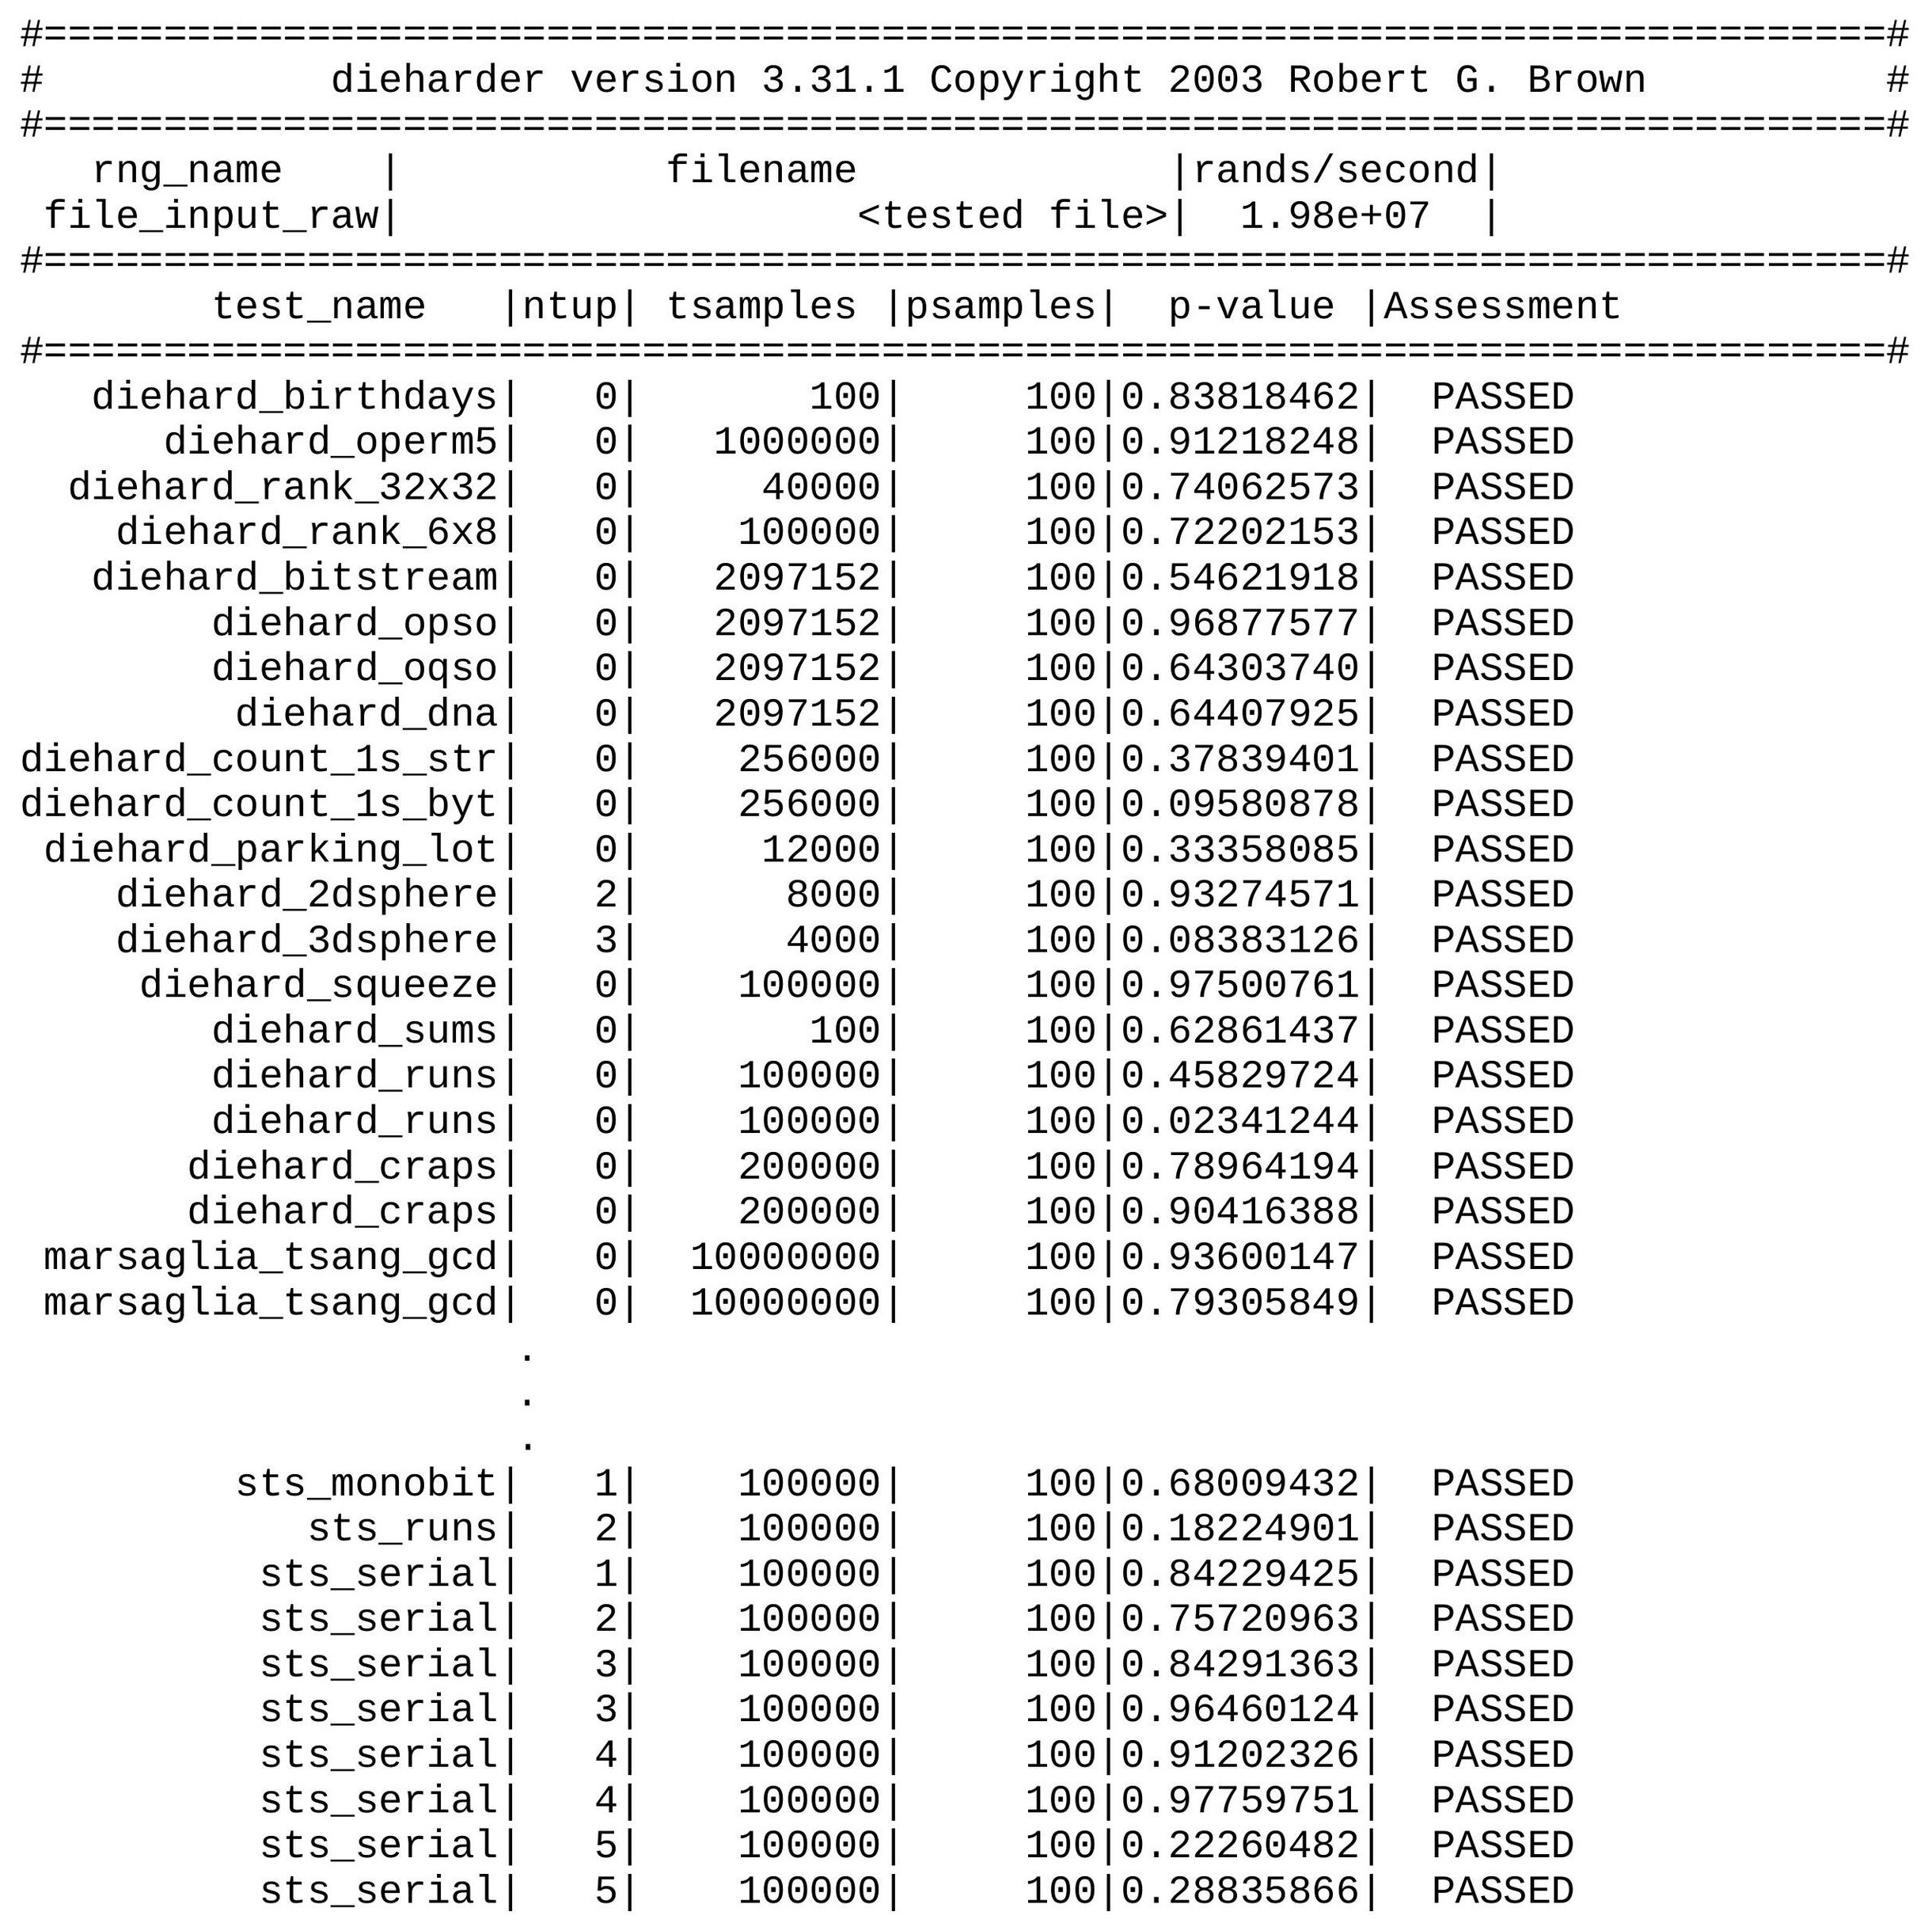
\includegraphics[width=12.5cm]{figures/outputs-appendix/dieharder.jpg}
  \end{center}
  \caption{Example of results table from the \emph{Dieharder} battery.}
  \label{fig:die_out}
\end{figure}

\pagebreak

\begin{figure}[h]
  \begin{center}
    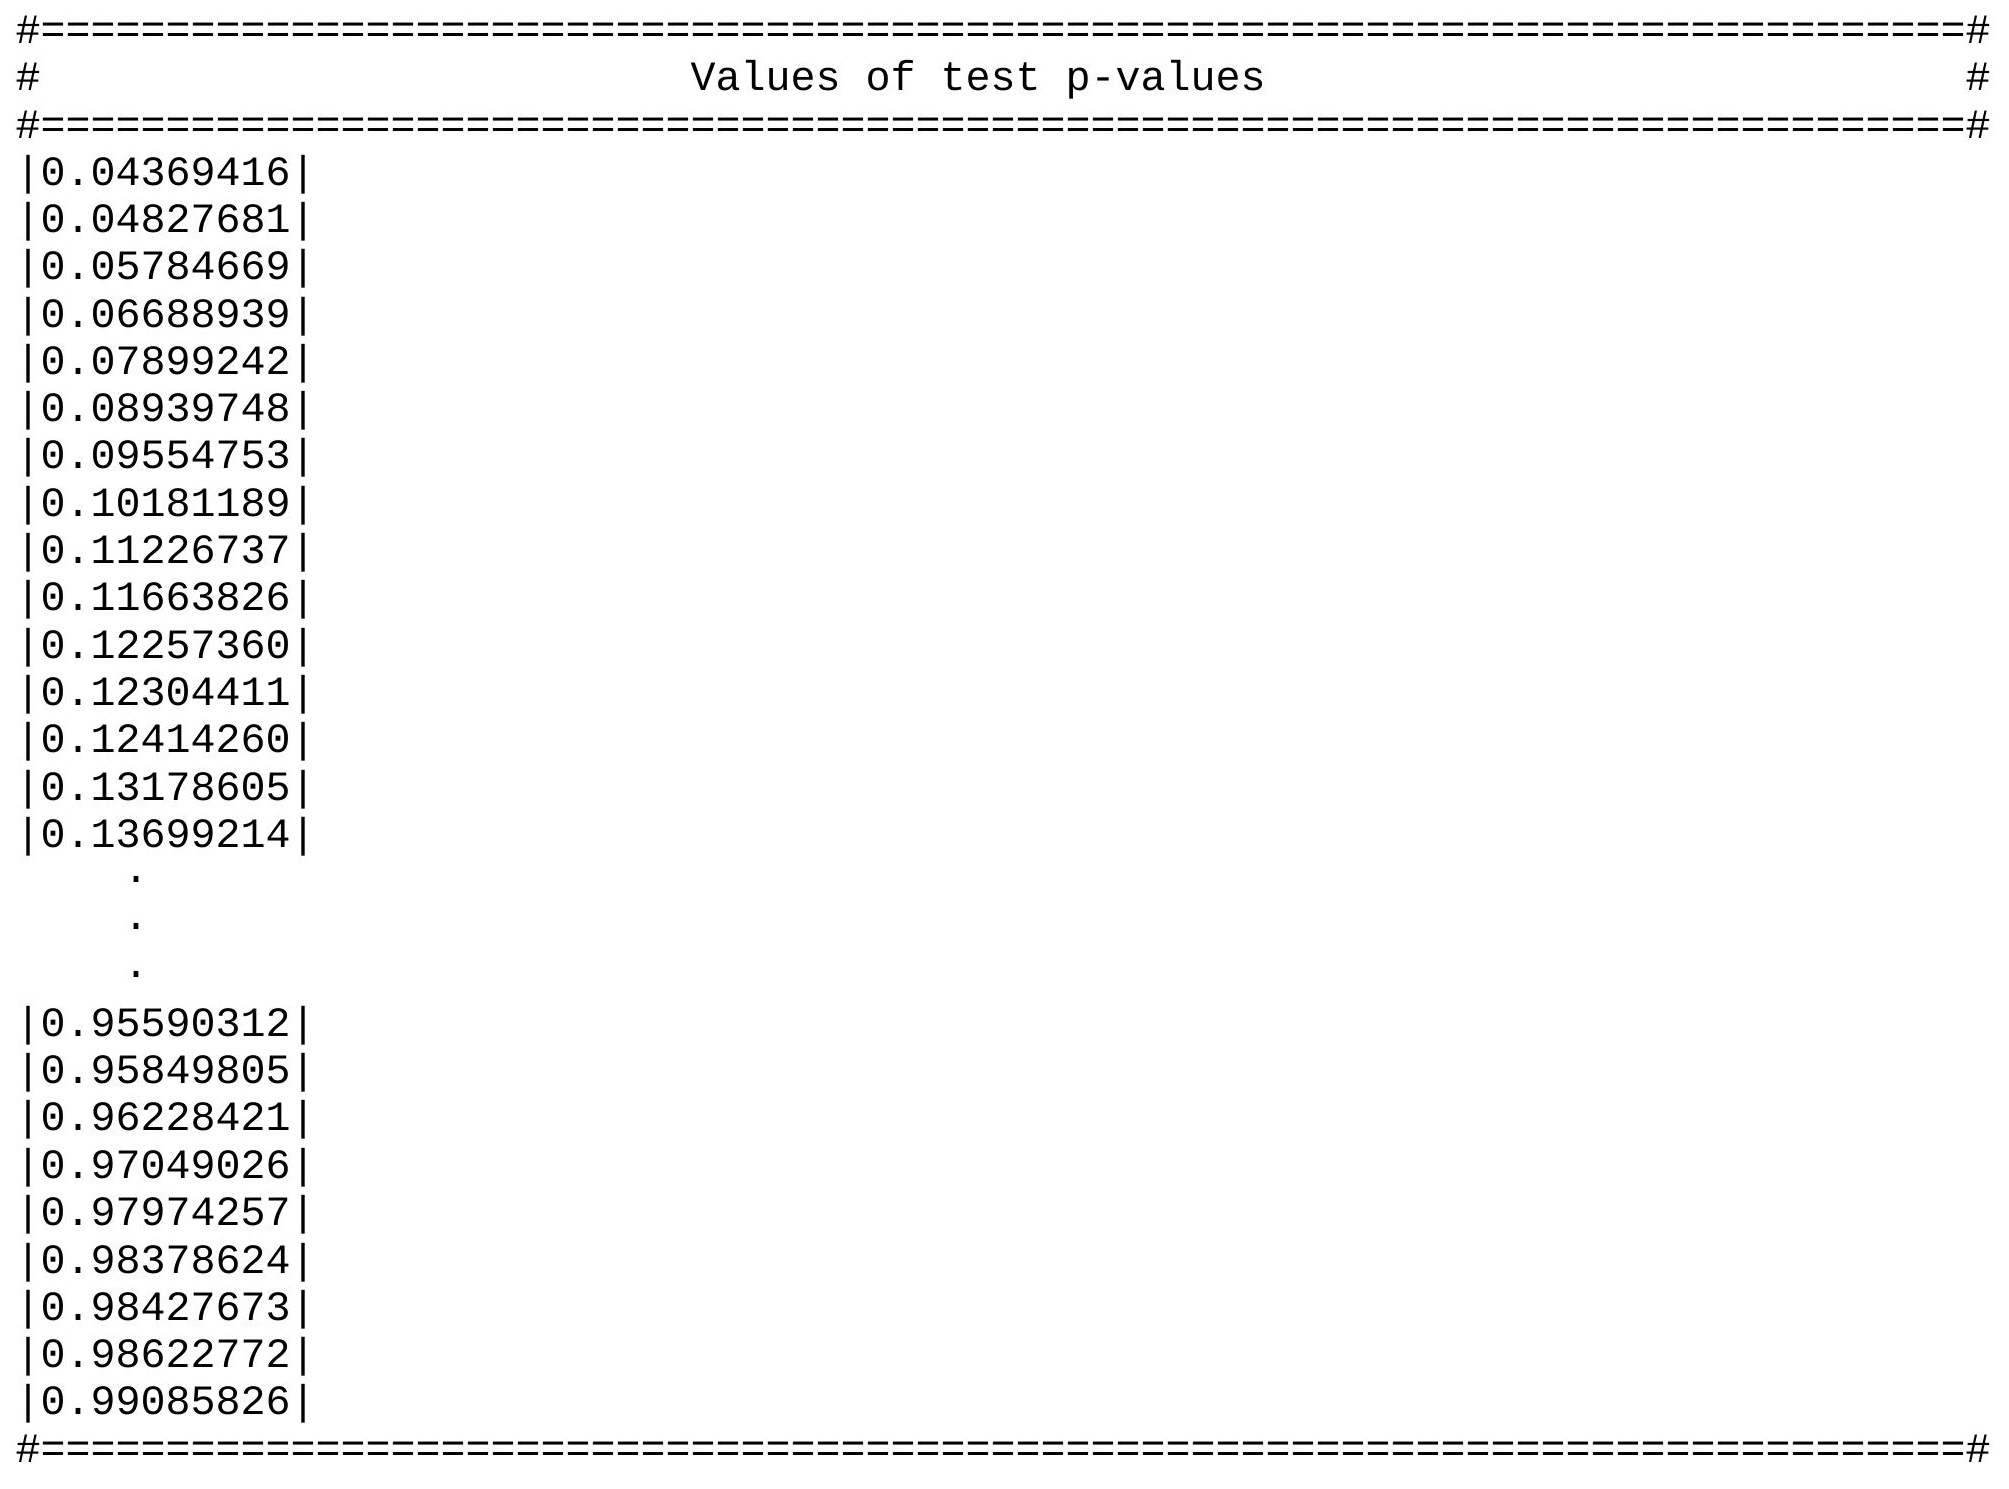
\includegraphics[width=12.5cm]{figures/outputs-appendix/pvals.jpg}
  \end{center}
  \caption{Examples of first-level p-values printout from \emph{Dieharder} battery}
  \label{fig:die_pvals}
\end{figure}

\pagebreak

\section{NIST STS output} \label{append:nist-output}
\begin{figure}[h]
  \begin{center}
    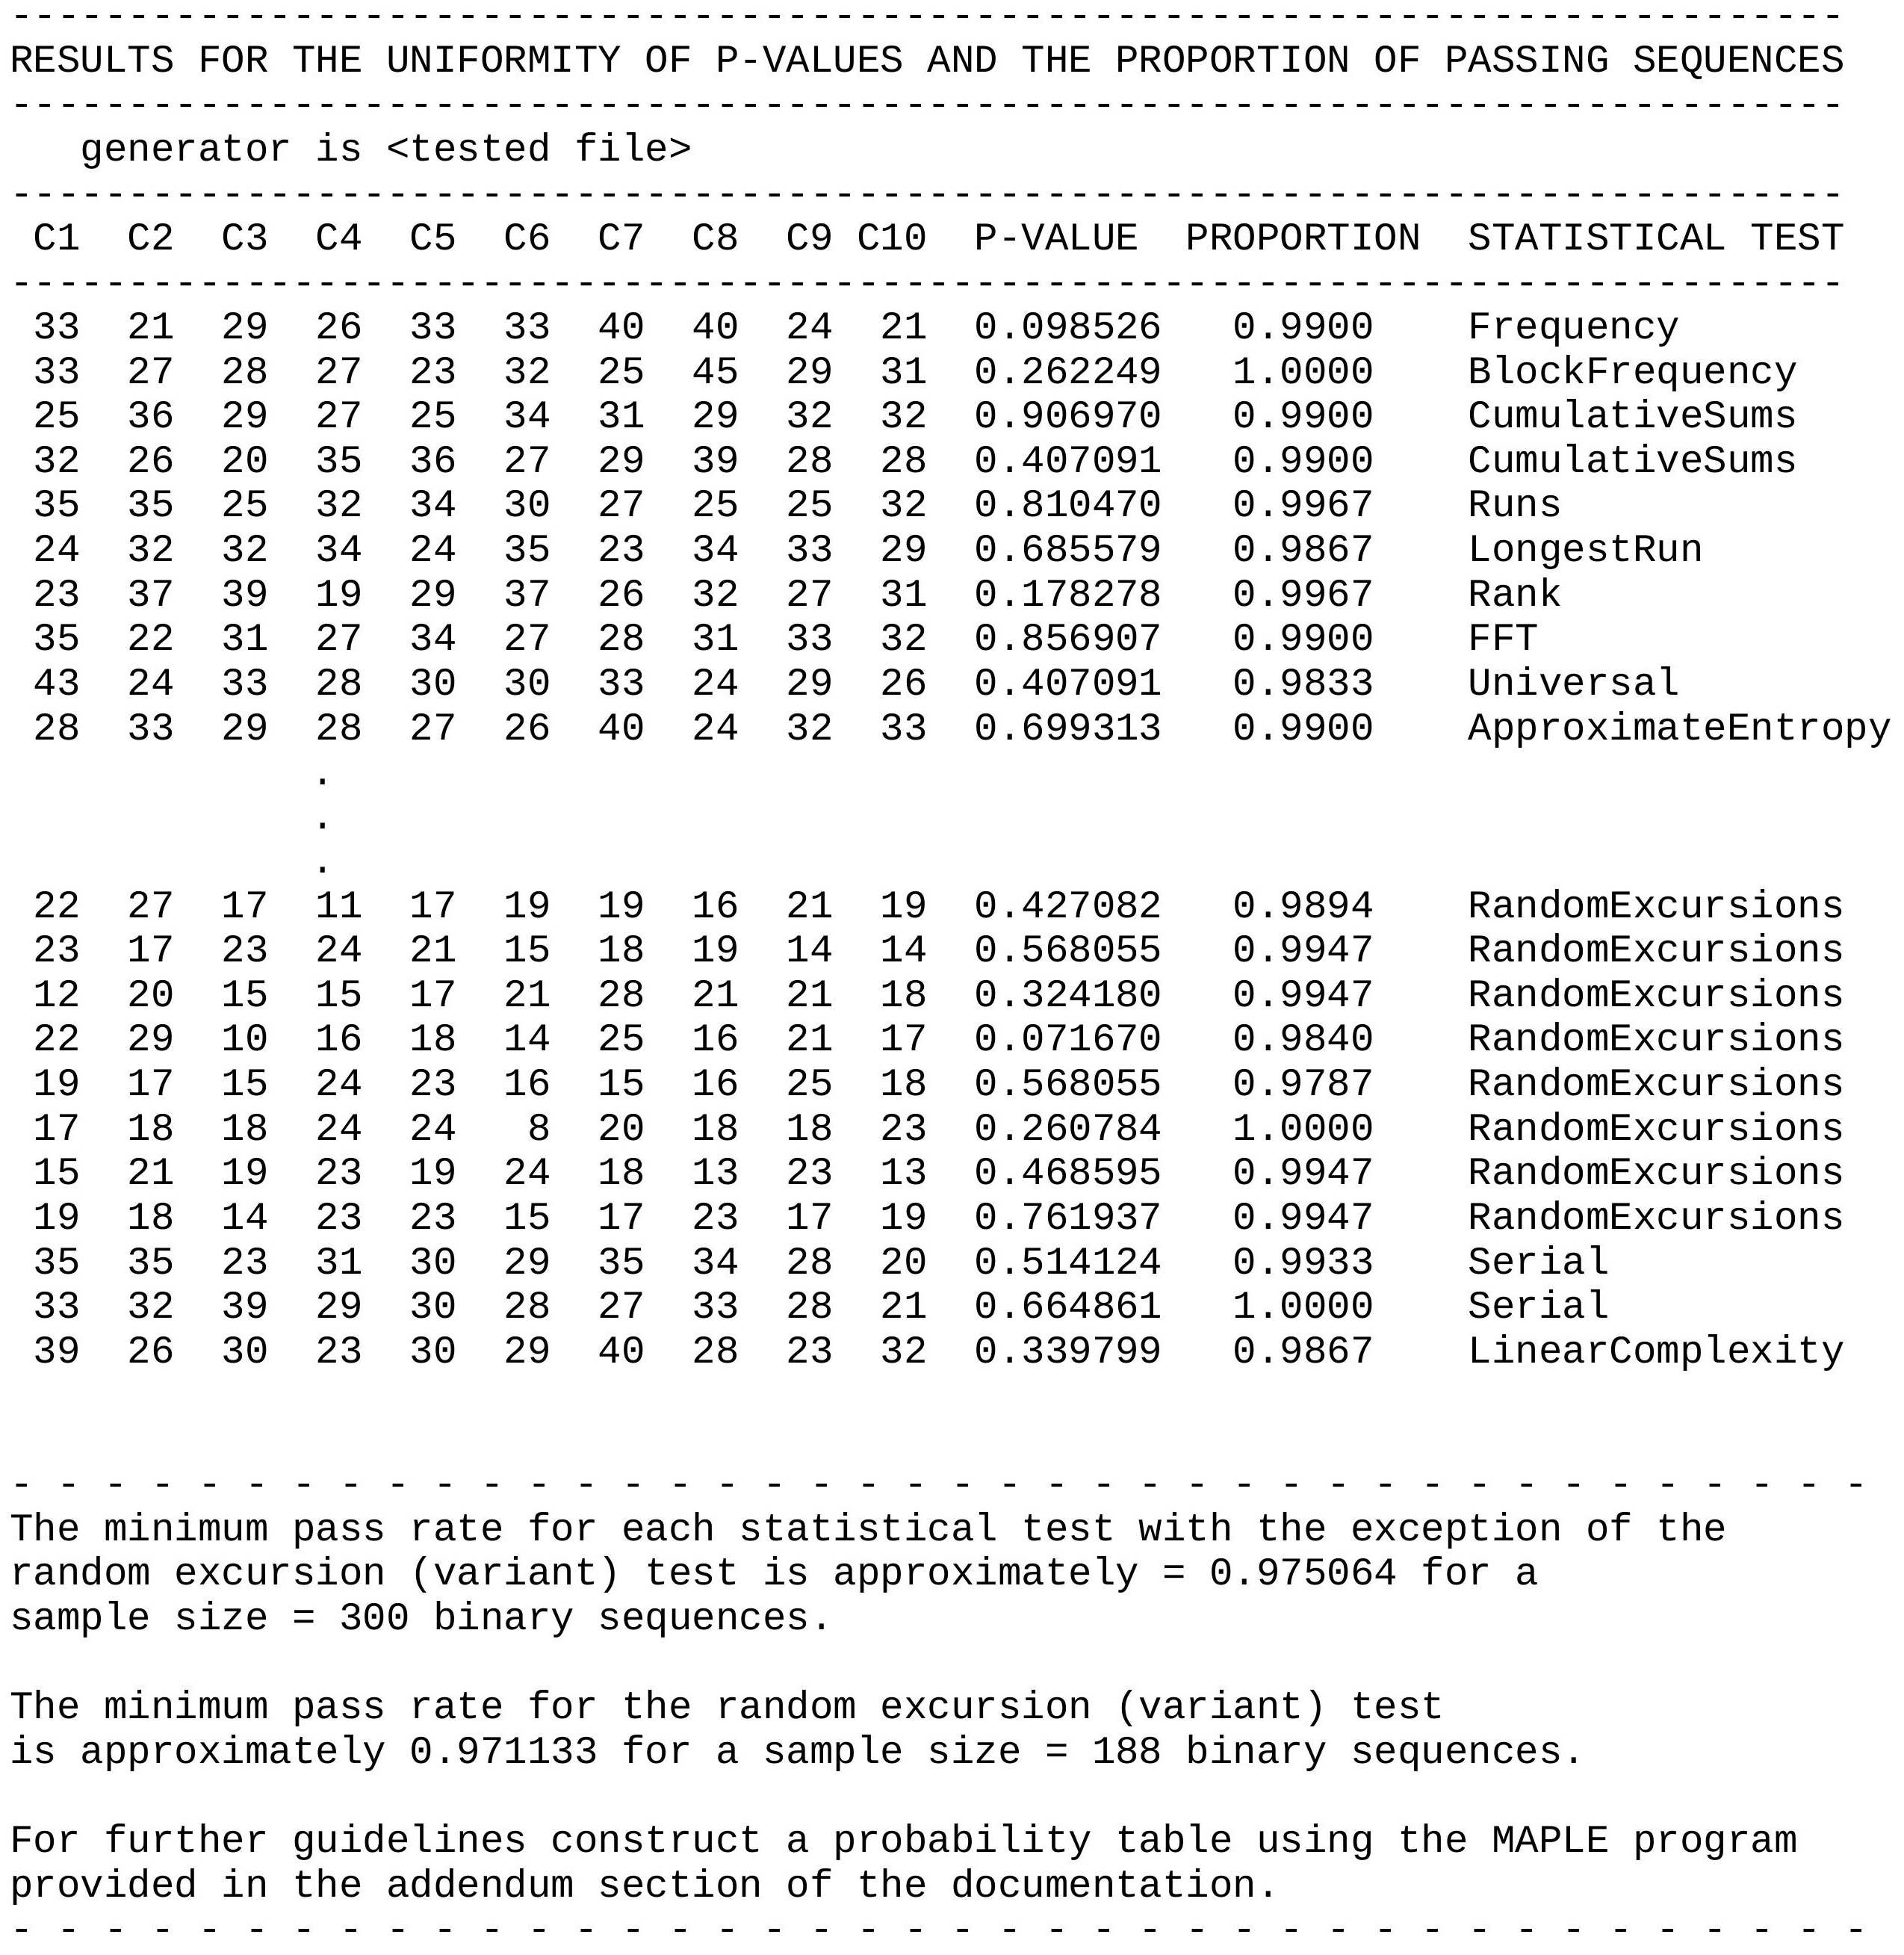
\includegraphics[width=12.5cm]{figures/outputs-appendix/finalAnalysisReport.jpg}
  \end{center}
  \caption{Example of results table from the \emph{NIST STS} battery.}
  \label{fig:nist_tab}
\end{figure}

\pagebreak

\begin{figure}[H]
  \begin{center}
    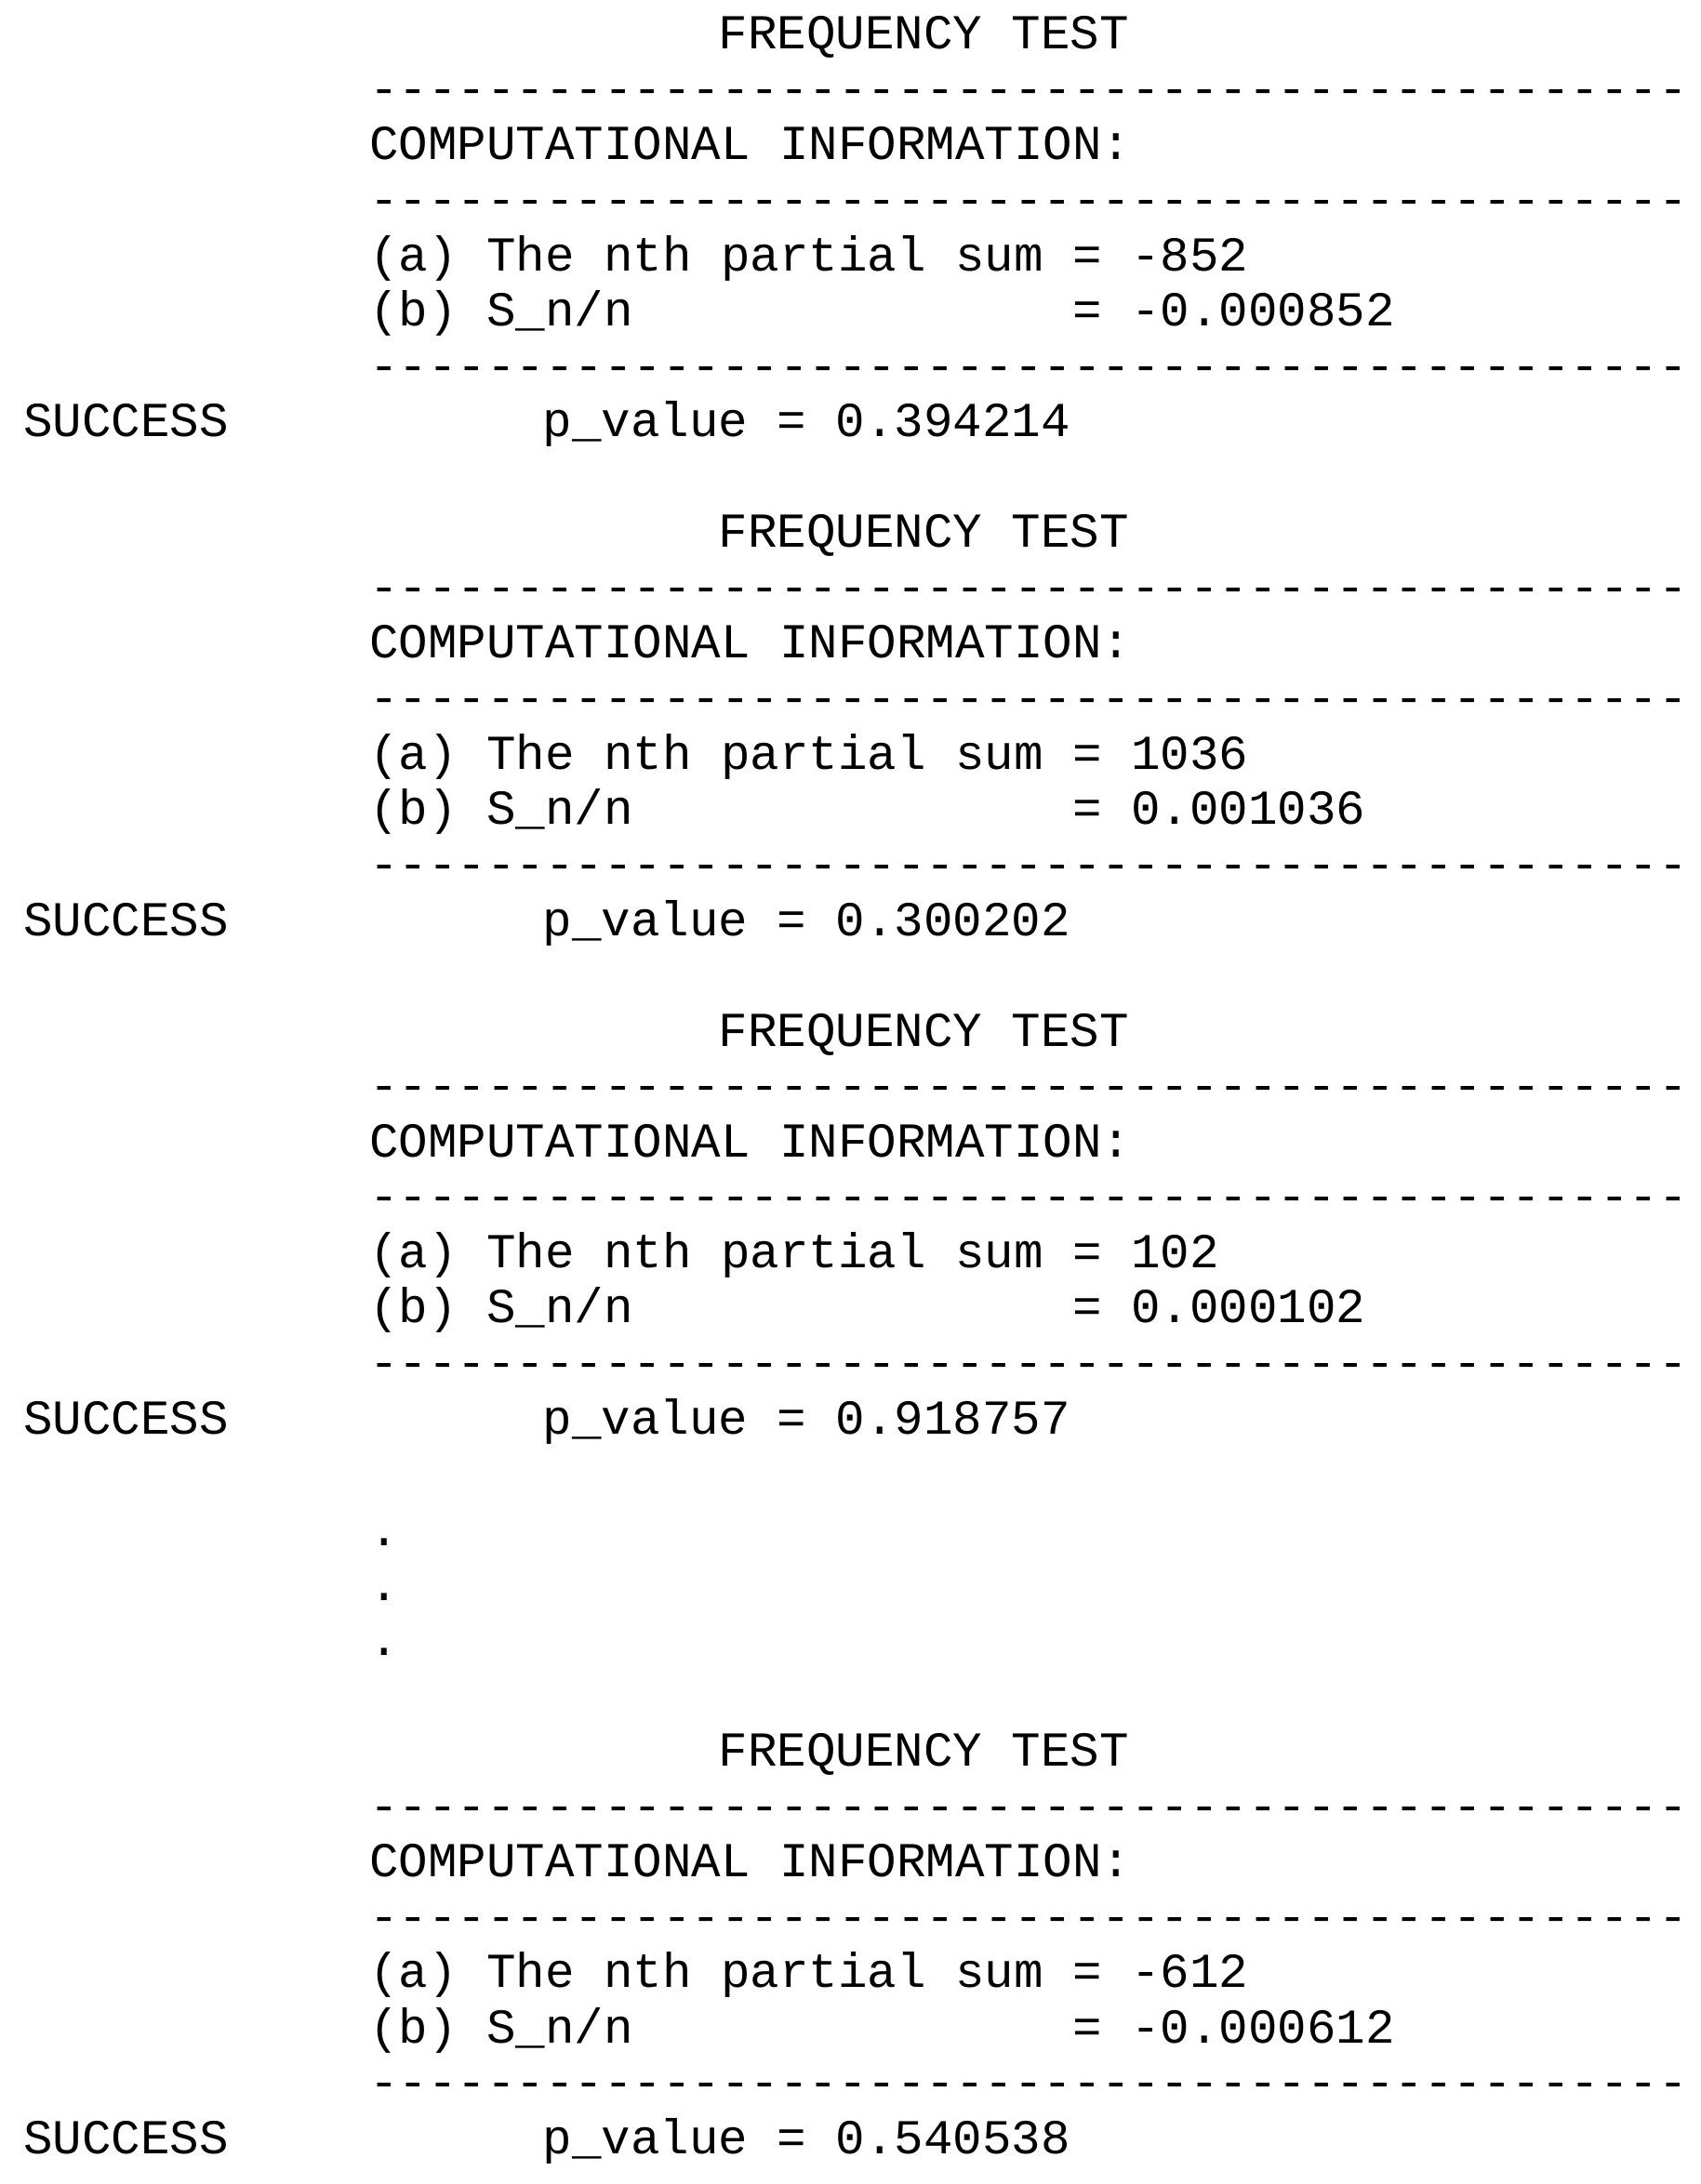
\includegraphics[width=9cm]{figures/outputs-appendix/stats.jpg}
  \end{center}
  \caption{Example of p-values, test statistics and other information from NIST STS's \emph{stats.txt} file.}
  \label{fig:nist_stats}
\end{figure}

\pagebreak

\section{TestU01 output} \label{append:tu01-output}

\pagebreak

\section{FIPS battery output} \label{append:fips-output}


\begin{figure}[h]
  \begin{center}
    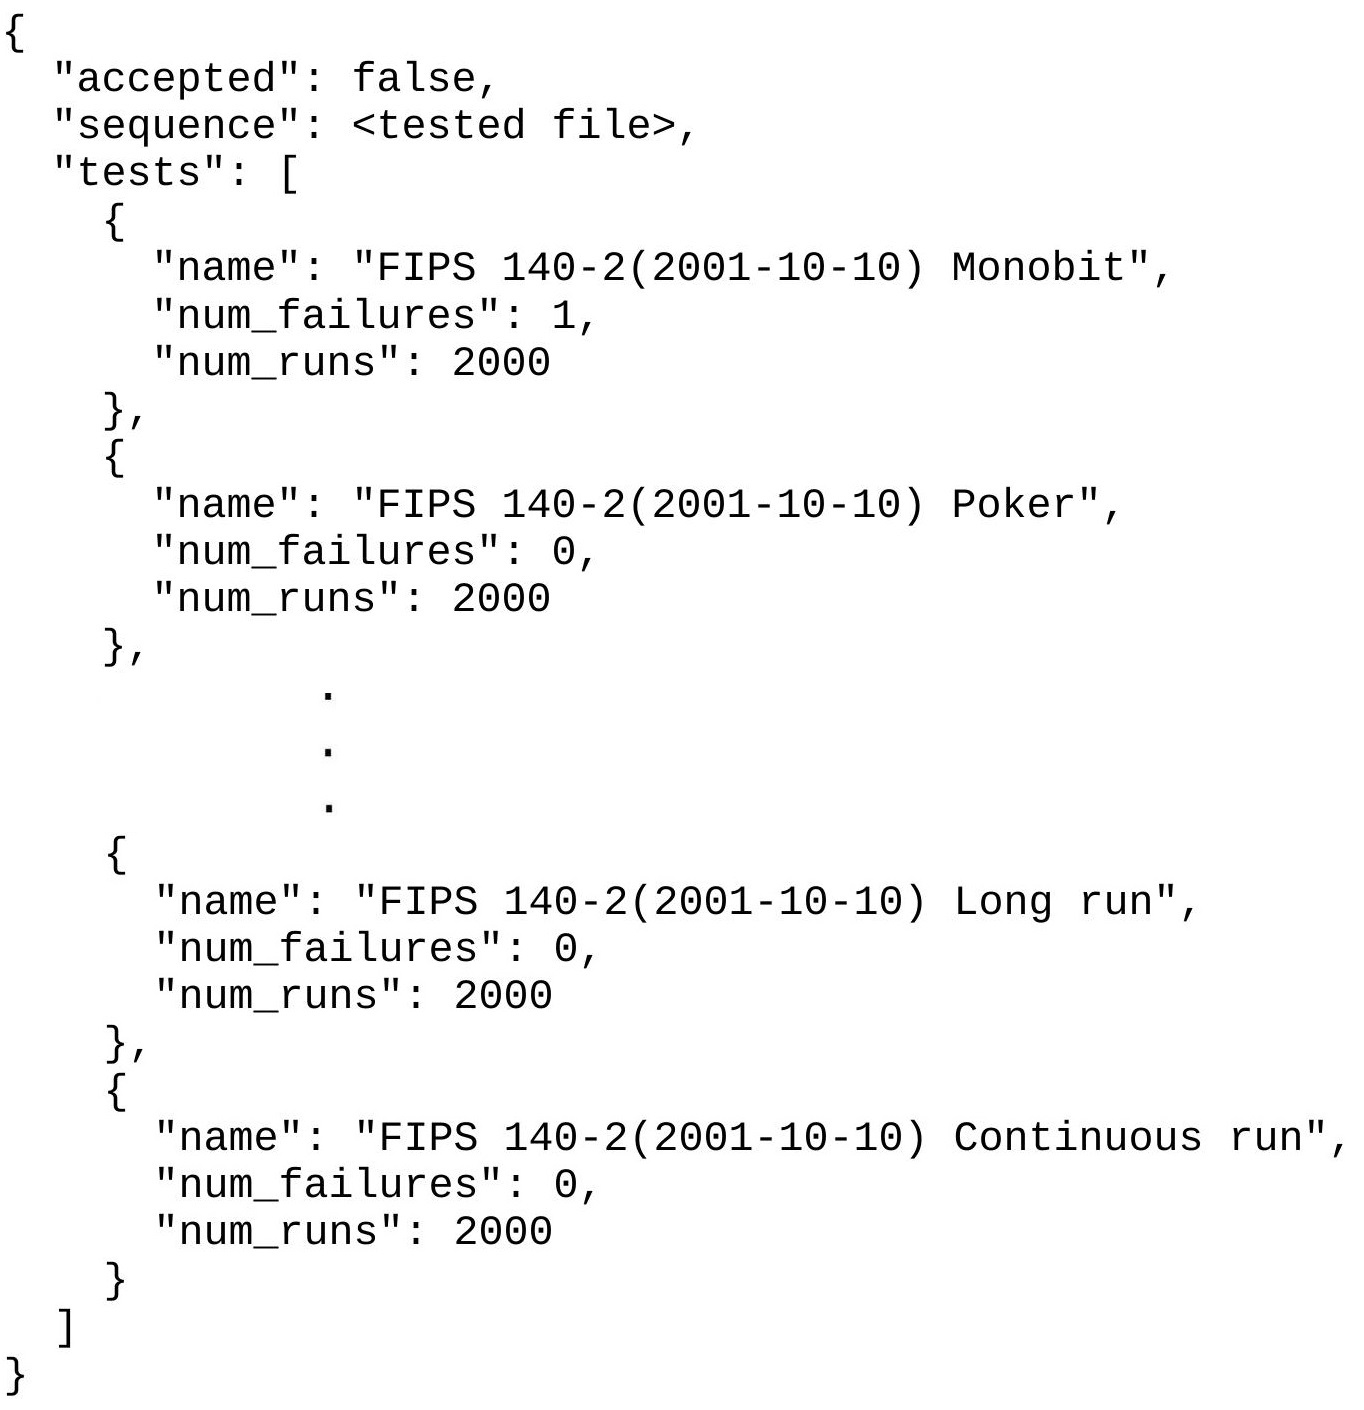
\includegraphics[width=10cm]{figures/outputs-appendix/fips.jpg}
  \end{center}
  \caption{Example of output from \emph{FIPS} battery.}
  \label{fig:fips_example}
\end{figure}

\section{BSI battery output} \label{append:bsi-output}


\begin{figure}[H]
  \begin{center}
    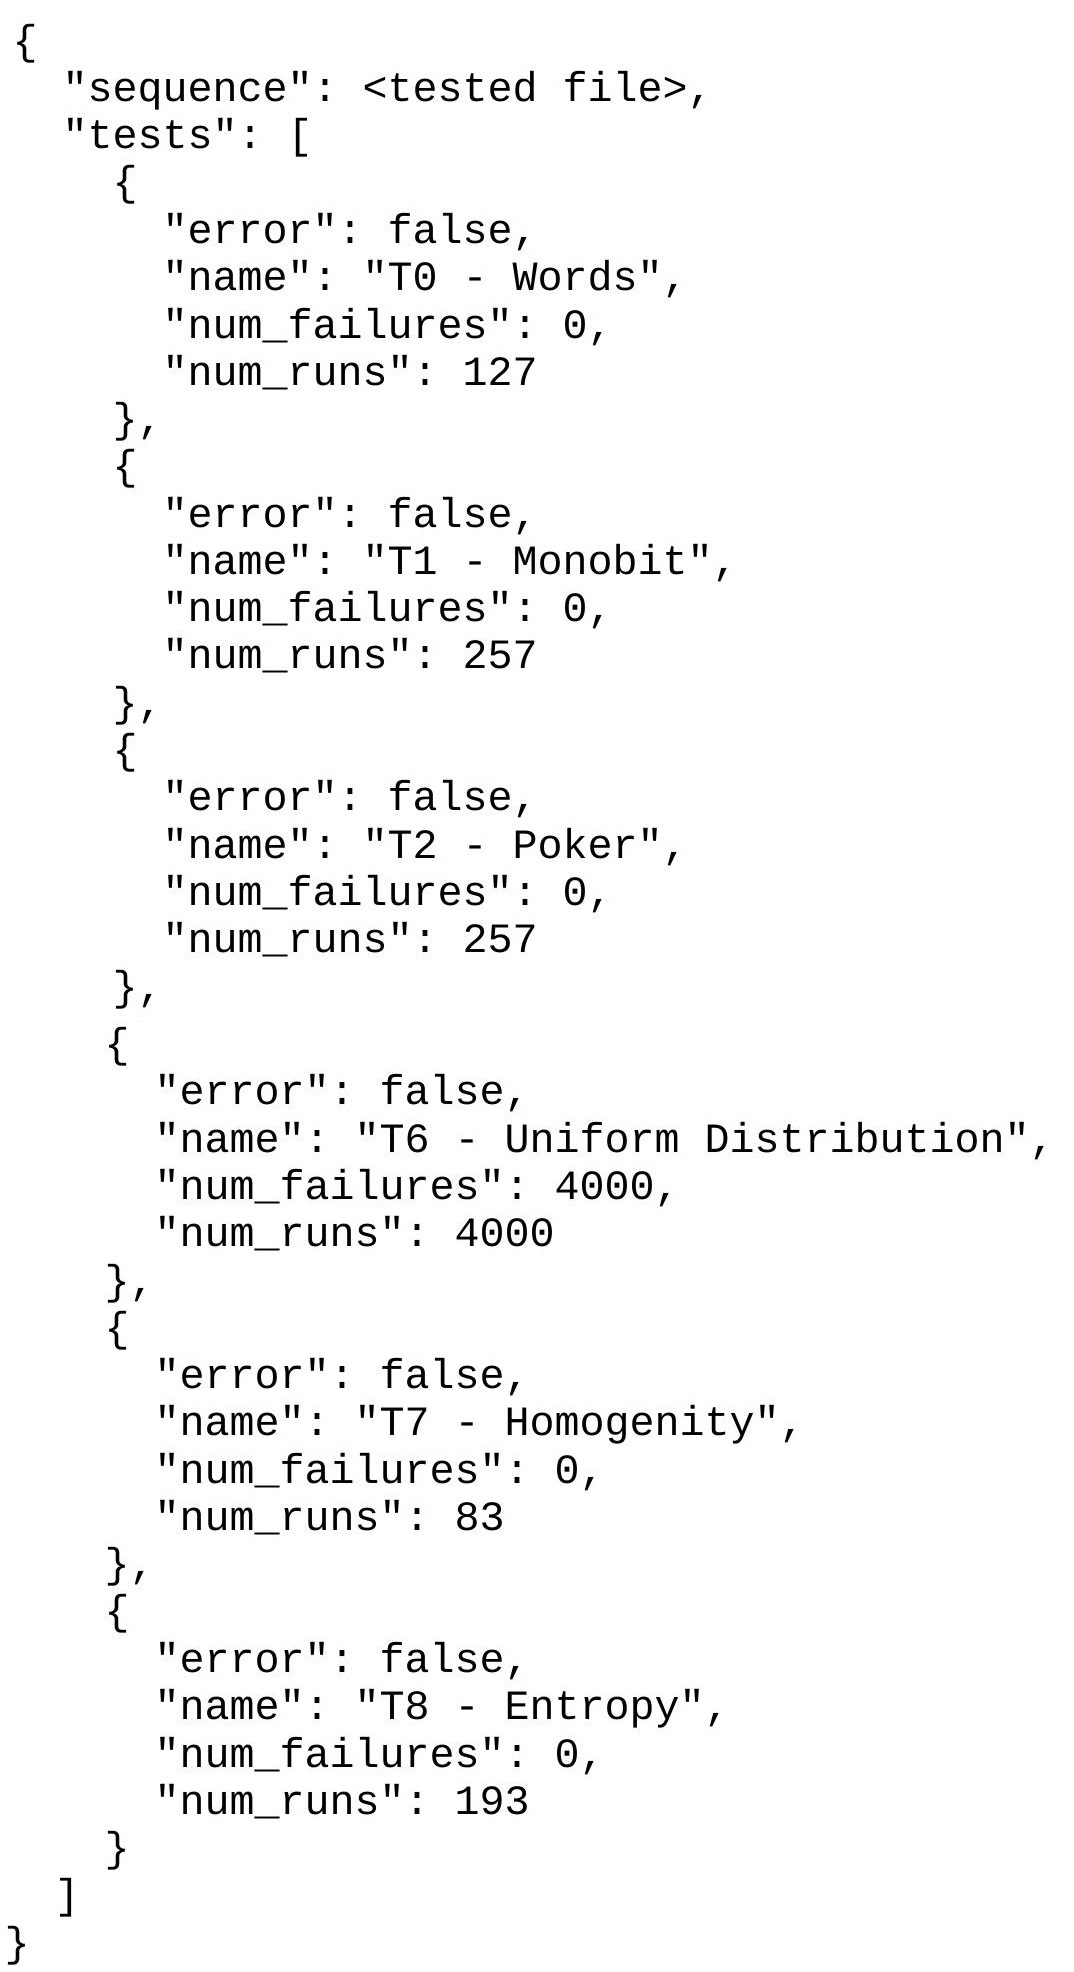
\includegraphics[width=7.5cm]{figures/outputs-appendix/bsi.jpg}
  \end{center}
  \caption{Example of output from \emph{BSI} battery.}
  \label{fig:bsi_example}
\end{figure}



\chapter{Testing Toolkits} \label{append:rtt}

\section{RTT settings}

\begin{figure}[H]
  \begin{center}
    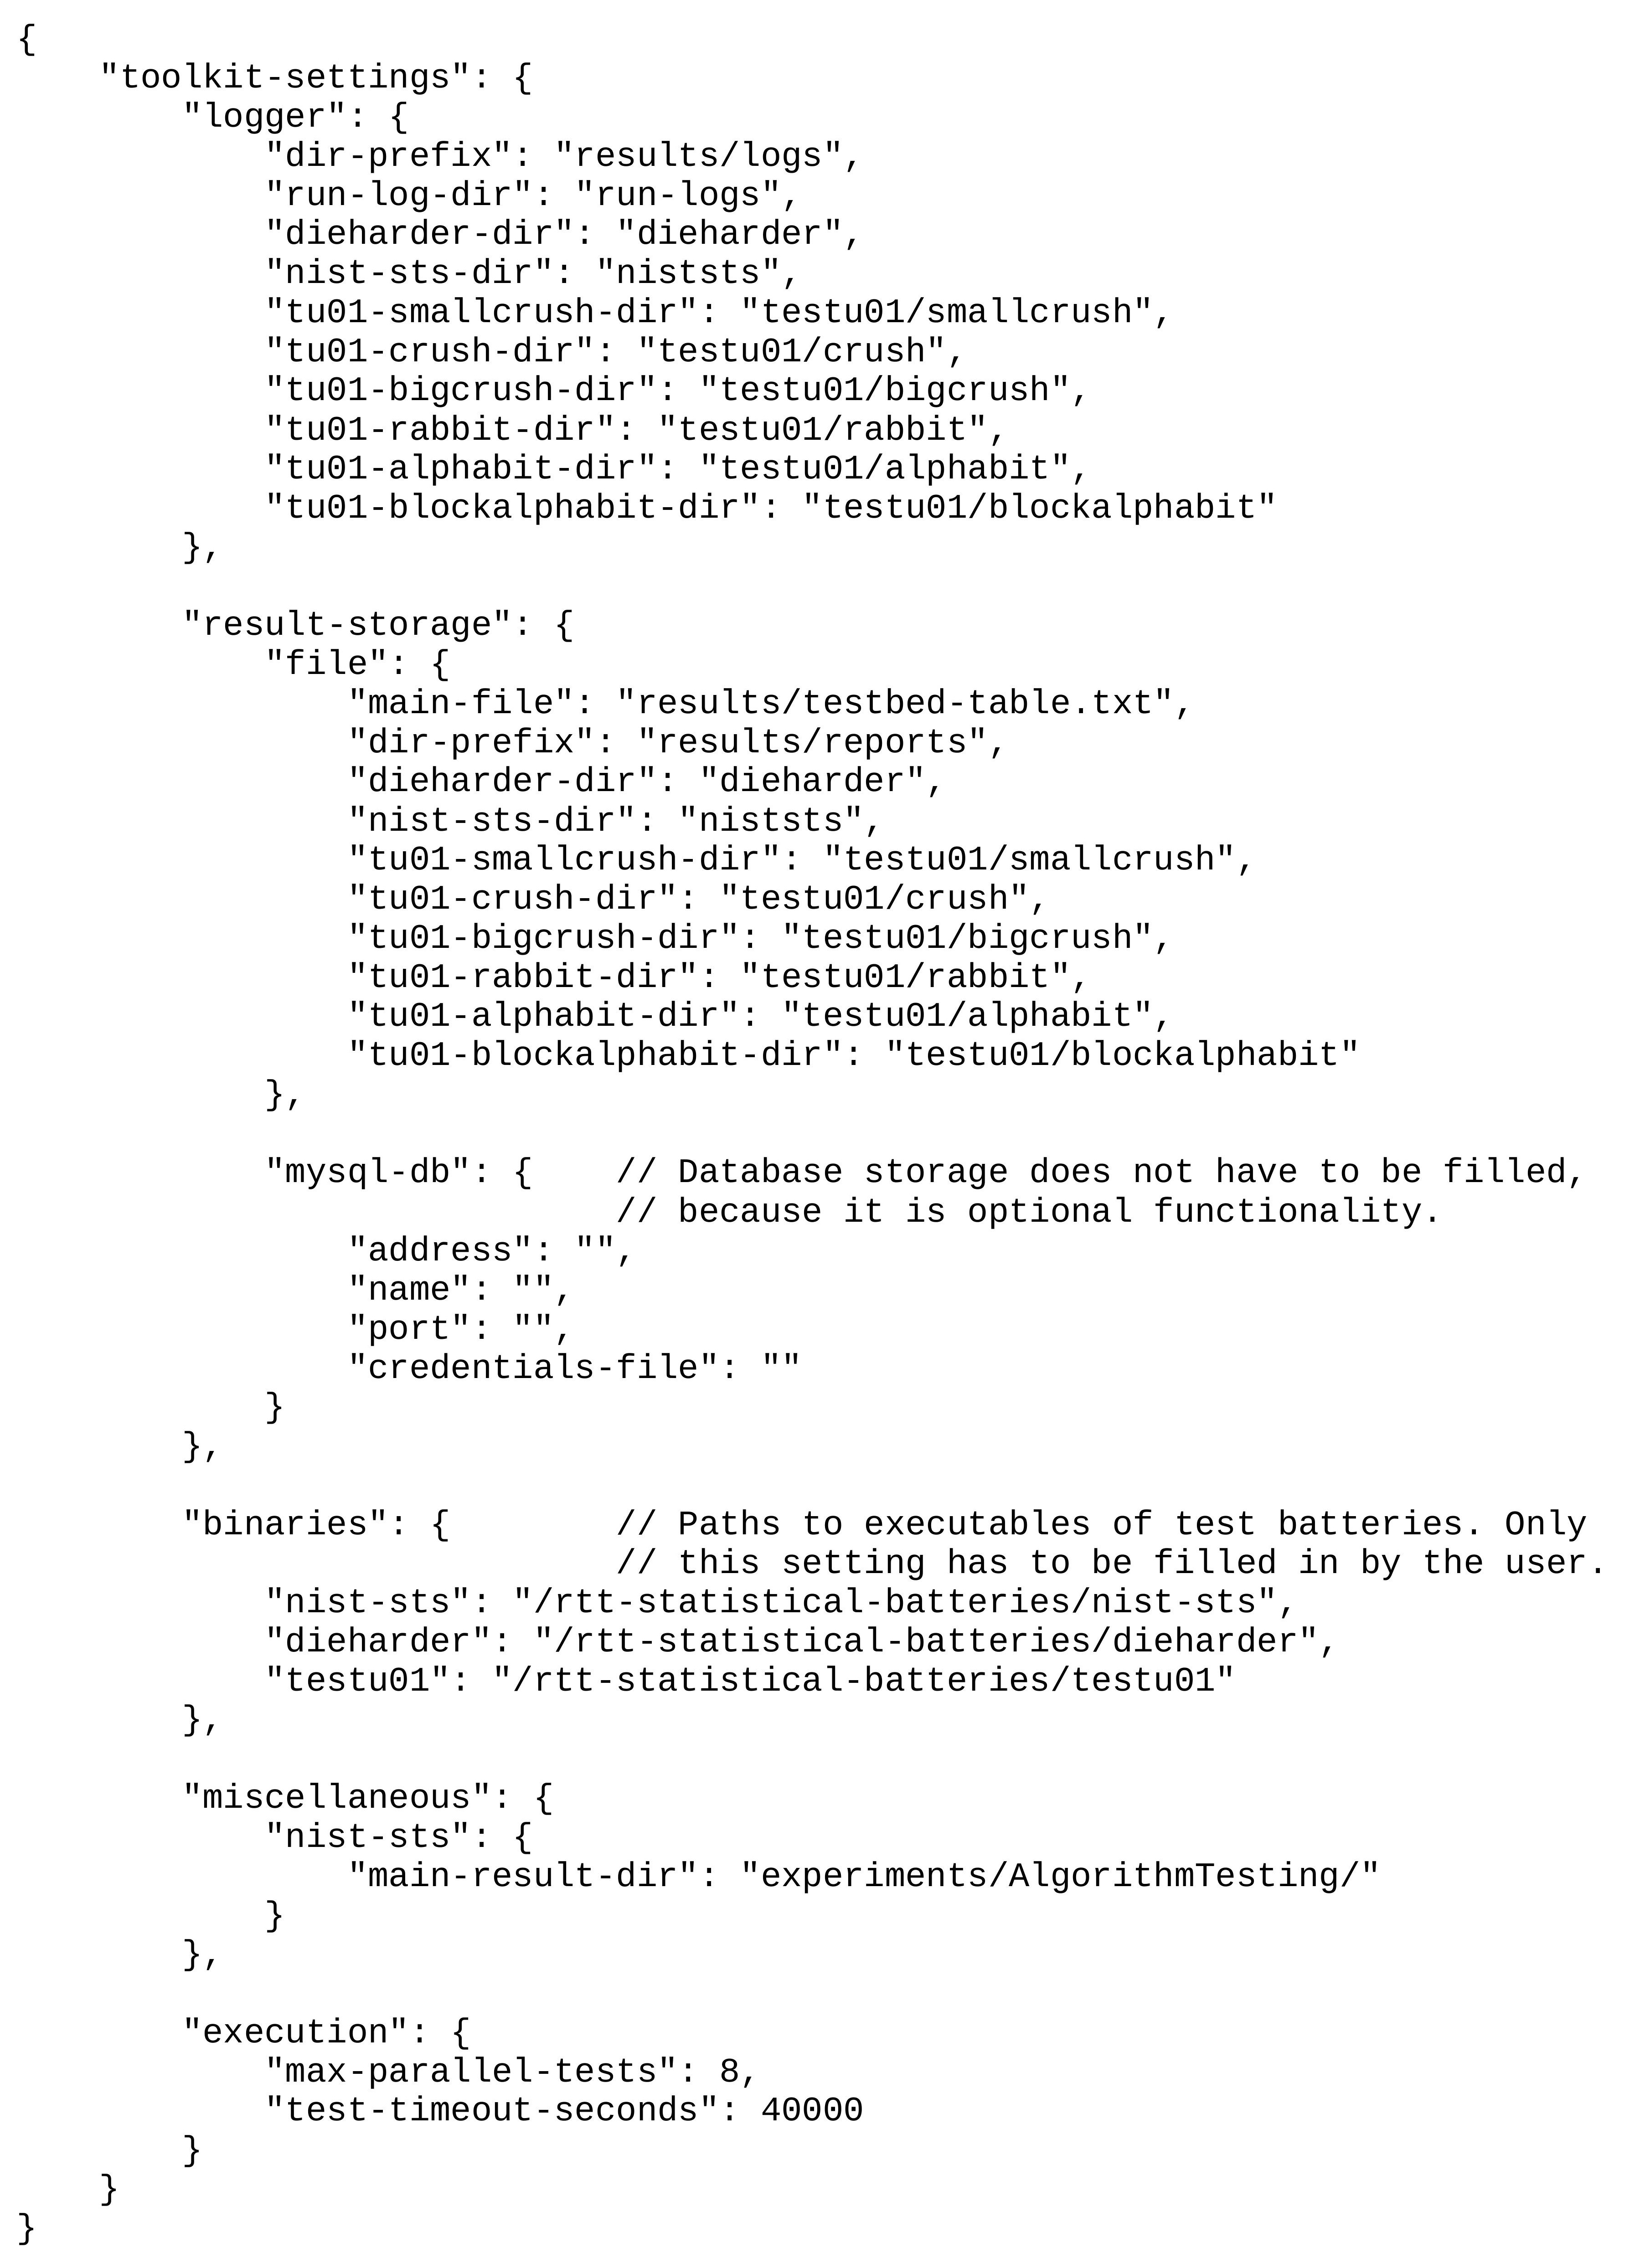
\includegraphics[width=11cm]{figures/rtt/rtt-settings.jpg}
  \end{center}
  \caption{General settings for \emph{RTT} stored in \emph{rtt-settings.json} file.}
  \label{fig:rtt_settings}
\end{figure}



\section{RTT battery configuration} \label{append:rtt-setting}

\begin{figure}[H]
  \begin{center}
    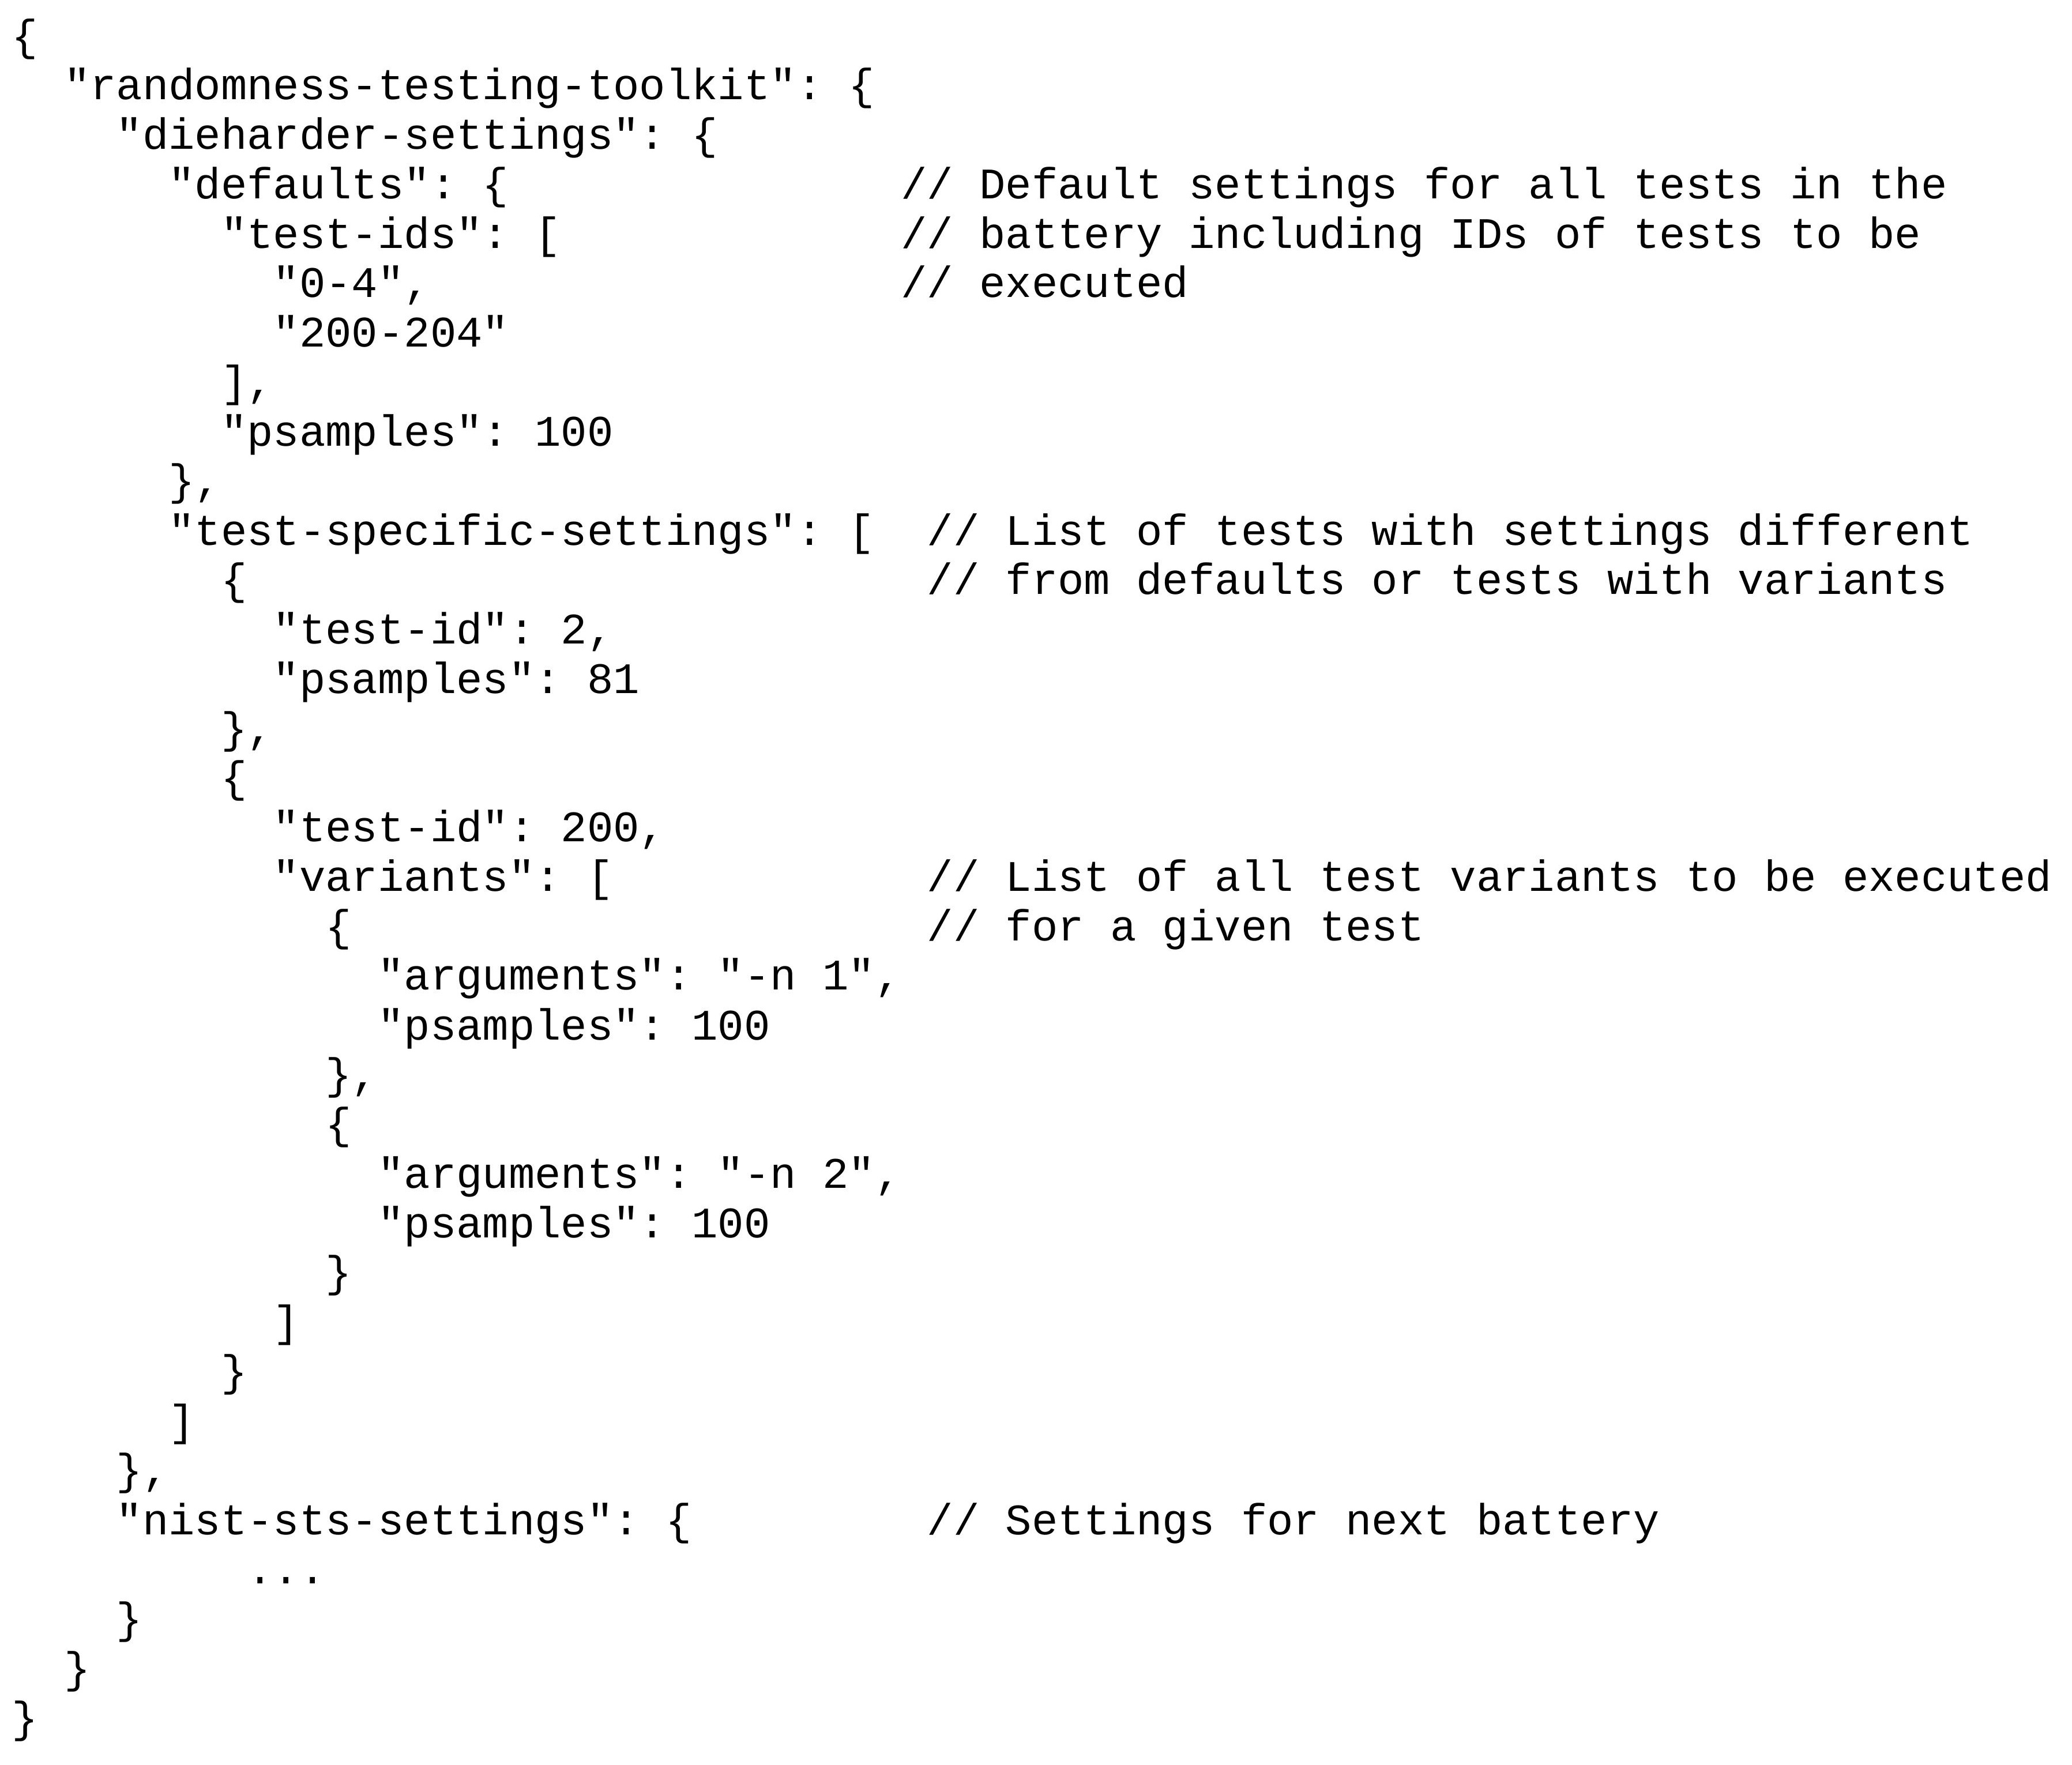
\includegraphics[width=12.5cm]{figures/rtt/config.jpg}
  \end{center}
  \caption{Example of battery configuration file for \emph{RTT}.}
  \label{fig:rtt_config}
\end{figure}



\chapter{RTT output} \label{append:rtt-output}


\chapter{rtt-py out} \label{append:rtt-py-output}
\end{document}
